\documentclass{article}[10pt]

\usepackage[utf8]{inputenc}

\usepackage{graphicx}
%\twocolumn
\usepackage[a4paper, total={6.5in, 10in}]{geometry}
\usepackage{setspace}
\onehalfspacing

\usepackage[notes,backend=biber]{biblatex-chicago}
%\usepackage{cite}
\bibliography{bib}

\usepackage{lscape} %allows landscape page

\usepackage{xcolor} % for the "DRAFT" header
\usepackage{fancyhdr} % for the "DRAFT" header
\pagestyle{fancy}

\DeclareRobustCommand{\bitcoin}{{%
  \normalfont\sffamily
   \raisebox{-.05ex}{\makebox[.1\width][l]{-\kern-.2em-}}B%
}}

\usepackage{amsmath}

%\usepackage[T1]{fontenc}
%\usepackage{lmodern}

\begin{document}


\begin{center}
    \color{red}
    Known areas for improvement
\end{center}

\begin{itemize}
    \color{red}
    \item Sections 2 and 5 through 10 are still in a brainstorm phase rather than being actual full fledged drafts
    \item It needs to be considered whether the unusual structure of Section 4 is helpful for comprehension or in need of rethinking.
    \item Section 3 needs elaboration and honing to ensure that the reader thoroughly understands all prerequisite concepts
    \item I'm not happy with the current footnote formatting. Need to figure out:
    \begin{itemize}
        \item How to clean up the look
        \item How to incorporate page numbers
    \end{itemize}
    \item Need to go through every sentence and rewrite it a few times to ensure:
    \begin{itemize}
        \item clarity
        \item conciseness
        \item consistent tense throughout. Also consistency elsewhere, such as point of view or lack of use of the oxford comma
        \item no unnecessary jargon or unreasonably difficult vocabulary that would hamper comprehension by a non-technical audience
    \item for all the terms I'm constantly confining, I need to establish consistent use of language including use of capital letters
    \end{itemize}
\end{itemize}

\newpage

\fancyhead{} % clear all header fields
\renewcommand{\headrulewidth}{0pt}
\fancyhead[R]{\color{red} \textbf{DRAFT}}

\title{Subsettable Enmeshed Cooperative Clusters ("SECCs"):\\
Incorporating Decentralized Information Into Firm Structure}
\author{Evin Tunador}
\date{\today}
\maketitle
\thispagestyle{fancy}

\begin{abstract}
    In this paper, I detail a potential meta-organizational structure for Decentralized Autonomous Organizations ("DAOs") that may allow humanity to partially bridge the gap between modern capitalist society and that of the socialist ideal, entirely through bottom-up information transfer and grassroots participation. 
    By allowing for the creation of easy-to-set-up, highly customize-able, modular, interconnected, and dynamic cooperative organizations, one can simultaneously circumvent many of the major flaws of late-stage capitalism and incorporate some of the theoretical benefits of socialism into an otherwise officially and completely free market society, all without any governmental participation. 
    Creating contracts, cooperatives, organizations, businesses, etc. on the Blockchain is not a new idea, but allowing groups with altogether separate functions to interconnect and exist as sub or super-structures to each other while changing structure dynamically to fit market circumstances may lead to a whole that is greater than the sum of its parts. 
    Designing highly-customizable group templates and creating a user interface simple enough for Blockchain-illiterate people to participate will encourage substantial levels of trial and error, thereby creating a landscape upon which different group parameters, types, structures and philosophies can compete. 
    By taking advantage of previously unutilized decentralized information and further using the naturally emergent survival-of-the fittest dynamic between groups as a partial substitute for and compliment to the price system, we can potentially fix many of the the inefficiencies intrinsic to a free market system and its closely related industries and institutions, in some cases by acting alongside them and in others by replacing them entirely. 
\end{abstract}

\vspace{0.5in}
\textbf{\color{red} note: The abstract is the one part of this paper where my goal is to create intrigue for a technical audience, specifically economists. In this sense it is not written to be easily understandable by those without said expertise}

\newpage

\begin{center}Author's Foreword\end{center}

\textit{Dear Reader,} \par 
\vspace{0.2in}

\textit{It is my opinion that research papers are generally overwritten with unnecessary jargon in order to gatekeep the subject matter and to make the author seem and feel more intelligent and important. 
These barriers to entry discourage the scientific process and hurt us all by extension. 
For this reason, I have elected to do my best at making this paper as accessible as possible. 
As such, you will notice a writing style that is often closer to that of narrative than traditional scientific papers, language that occasionally borders on the informal, and a slightly unusual organizational structure. 
I apologize if any of these deviations from the norm turn out to be unnecessary or even counter-productive. } \par

\textit{Similarly, readers with technical expertise may find this paper to leave many avenues untraveled and questions unanswered. 
To you, I also apologize, but hope that you can appreciate my reasoning and motivation. 
For the economists in the crowd, rather than redefine the mathematical model of the firm and search out the equilibrium derivation presumably awaiting us above the clouds, I chose to keep my discussion of these new economic dynamics entirely descriptive with the exception of some footnotes. 
To get a handle on my motivation here, please see the various works of Friedrich Hayek, Benoit Mandelbrot and especially Nassim Nicholas Taleb. 
As to explicit methods of implementing my idea on the blockchain, I hope that those more knowledgeable than I in the art feel it worth their time to fill in those gaps.
On this last point, I would also like to acknowledge that my elementary understanding of cryptography, the blockchain, and computer programming in general leave open the possibilities for parts of or even the entirety of my idea to not be feasible, or to have already been proposed or even implemented. 
If anything, I perceive these scenarios as more likely than not. 
I will defer to the collective feedback I receive as a final judgement of this paper's merit.} \\

\textit{Thank you,}\par
\textit{Evin Tunador}

\newpage
\tableofcontents
\newpage

\noindent \textcolor{red}{Necessary Prerequisites:}
\textcolor{red}{\begin{itemize}
    \item switching to cooperative (profit-sharing) incentive structures
    \item a good standardized codebase for the DAOs to work within
    \item a user interface easy enough to be accessible to the general population
\end{itemize}}
\textcolor{red}{Breakdown of Ideas:}
\textcolor{red}{\begin{itemize}
    \item the firm as a fluid, ever-changing entity with many dimensions to vary upon
    \item organizationss as sub or super structures to each other rather than individual contractual agreements, specifically in the labor market
\end{itemize}}

\section{Introduction}
\label{section:Introduction}
In Section \ref{section:Motivation} I lay out the concerns that put me in the state of mind to have this idea and write this paper.
My hope is that it makes you, the reader, more open to the possibility of change. 
In Section \ref{section:Background} I summarize the bare minimum information needed to understand the rest of the paper. 
If you already consider yourself knowledgeable on the title of any subsections therein, please feel free to skip. \par 

In Section \ref{section:TheBasicIdea} I begin by describing the motivation and business model of two Subsettable Enmeshed Cooperative Clusters ("SECCs") in order to establish concrete examples to work off of. 
Then in Subsections \ref{section:TheBasicIdea}.X through \ref{section:TheBasicIdea}.Y I go through each feature of a SECC in detail, using the two examples to ground my discussion.
It is my hope that this unusual essay structure assists in comprehension and broad accessibility of the idea. \par 

In Sections \ref{section:CentralFlaws} and \ref{section:FreeFlaws} I attempt to convey the potential of SECCs to somewhat bridge the gap between socialism and capitalism by improving on and incorporating the best of both. 
This is a difficult endeavor for anyone to undertake without triggering deep tribal instincts if you happen to emphatically prefer one over the other.
All I ask of you is to keep an open mind.
This means that rather than seeing me as an enemy attacking your view of the world, please try see me as a friend attempting to brainstorm a solution to problems we all face.
Please be willing to be honest about the flaws of whichever economic system you consider to be your home team.
No one system system will ever be perfect, including the one I propose here. \par 

In Section \ref{section:Brainstorm} I've aggregated thoughts of mine that did not fit well into other sections even as footnotes, or that I just could not wrap my mind around well enough to write anything conclusive about. 
In Section \ref{section:Issues} I explore some of the potential counterarguments to my opinion that SECCs are the future.
Many consist of potential ideas and implementations for SECCs.
Finally, Section \ref{section:Conclusion} contains my concluding remarks.


\section{Motivation}
\label{section:Motivation}

\textcolor{red}{this section is extremely important. 
I need to really spell out the impending doom of the current system. 
properly lay out each problem in a convincing manner. and them go into how people who are *too* pro-capitalism have gotten dogmatig and they need to loosen up a big and face up to the fact that capitalism can't go *literally* forever so there will need to be something new at some point. 
to posit that you're at the apex of history is naive, narcissistic, moronic, etc and only serves to increase the chances that you do yourself harm through your insistence to maintain convention. 
that is not to say you have to regress to ideas that have already failed, like commumism, but it is to ask that you read this document as if what I'm proposing is something new entirely, and as such approach it with an open mind.} \\

\textcolor{red}{*Section needs to be rewritten*} \\
\textcolor{red}{here's what i'm thinking for organization:} \\
\textcolor{red}{\begin{itemize}
    \item American dream is crumbling (late-stage capitalism?)
    \begin{itemize}
        \item wealth inequality
        \item median income stagnation
        \item decreasing socioeconomic class mobility?\footnote{
            \textcolor{red}{need to confirm if true}}
        \item each generation no longer gets richer
    \end{itemize}
    \item alternatives are showing potential in that they have an altogether different set of strengths \& weaknesses
    \begin{itemize}
        \item china = communism + markets \& investment
        \item europe = democratic socialism?
        \item they seem to be on an improving or at least interesting path by some metrics, but haven't quite figured it out either
    \end{itemize}
    \item what if we instead look for an out of the box solution? - marx \& hayek both wanted a new system to facilitate information transfer in government\footnote{
        \textcolor{red}{I think i can find the source somewhere in the cryptocommunism book}\\
        \indent \indent \fullcite{alizart}}
\end{itemize}}

\textcolor{red}{Not sure how confident I am in this opinion, both its effectiveness and its feasability:}\\
\textcolor{red}{\textit{I need to downplay this metaphor to communism i tend to use. 
instead of a battle between capitalism and communism, i need to convey this as the next progression of the thing after capitalism in order for it to be convincing. 
the socialists will see the similarities on their own.}} \\


\section{Background}
\label{section:Background}

\textit{Section Notes:}\\
\textit{It is my hope that this section is sufficient to bring someone with absolutely zero knowledge about blockchain technology and little more than a vague awareness of economic concepts fully up to speed.}


\subsection{What is a Cooperative?}
\label{subsection:cooperative}

\textcolor{red}{\textit{Subsection Notes:}}
\textcolor{red}{\begin{itemize}
    \item \textit{maybe mention that girl from tiktok who started a company that pays all workers equally to demonstrate the growing cultural interest in the topic}\
    \item \textit{Not sure how in-depth I should get in this section. Maybe full on models of the cooperative firm in the footnotes? Do I need to discuss top-down corporations in detail to provide a point of reference for comparison, or is the novelty and utility of the cooperative structure obvious?}
    \item Doing both the Nembhard quote and the written definition is redundant. Need to decide which I prefer. Probably the latter and then I should go into more detail
\end{itemize}}

\textcolor{red}{\textbf{CONSIDERING REMOVING THIS SECTION AND ALL MENTION OF COOPERATIVES ENTIRELY}}

\begin{quotation}
\textit{[Cooperatives] use a sense of solidarity and concern for community to promote economic alternatives that create economic growth and sustainability. At the same time, their solidarity and collective action increase productivity and help stabilize their economic circumstances. Moreover, cooperative economics is often viewed as a tool or strategy of a larger movement toward the elimination of economic exploitation and the transition to a new social order.} \\
\textit{- Jessica-Gordon Nembhard \autocite{nembhard2021collective}}
\end{quotation}

According to the International Cooperative Alliance, "[c]ooperatives are people-centred enterprises owned, controlled and run by and for their members to realise their common economic, social, and cultural needs and aspirations."\autocite{ica}
They exist in a variety of forms as an alternative to organizations built on top-down power and incentive structures. 
Their goals often consist of some combination of fairness, profit-sharing, equality, and/or social-justice.\autocite{ica}
Much work has been done to study theory and evidence behind the structural benefits of cooperatives, both for their members and for the economies and ecosystems they exist within.\autocites{nadeau2012cooperative,potashev2021mathematical,coopWhitepaper}
Some advantages outside the obvious include better weathering of recessions,\footnotemark \textcolor{red}{...}, and \textcolor{red}{...}.
    \footnotetext{\textcolor{red}{talk about that one in spain \& how it weathers recessions better. maybe talk about how classical econ theory posits that recessions would go better if workers were willing to take a decrease in wages instead of having some people fired?}}\par






\subsection{Blockchain - How it Works}
\label{subsection:blockchain}

Blockchain refers to a technology invented by Satoshi Nakamoto (a pseudonym; the author is anonymous) as a response to the 2008 financial crisis, with the first instantiation being the cryptocurrency Bitcoin (denoted "\bitcoin").\autocite{nakamoto2008bitcoin} 
It essentially consists of an online list of transactions and interactions commonly monitored by many people that uses cryptography (fancy math) to ensure that no one can lie about a transaction. 
Whereas a traditional financial ledger needs a single point of contact to verify the legitimacy of transactions, such as a bank, blockchain ledgers do not have to be owned or operated by a single party. 
Instead, they are decentralized meaning that their legitimacy comes from the common consensus of everybody using the ledger rather than one powerful entity getting to define the truth.\footnote{
    \fullcite{blockchain101}\\
    \indent \indent \textcolor{red}{Need to double check that this source actually fits. I just selected it cuz it was in the bibliography but I don't actually remember reading it}} \par

Over the past 14 years, blockchain technology has spawned innovations including cryptocurrencies (generally denoted "\textcent"), non-fungible tokens ("NFTs"), smart contracts, and decentralized autonomous organizations ("DAOs"). 
According to many reputable thinkers across industries and disciplines, some of these blockchain technologies have potentially revolutionary potential.\footnote{
    \textcolor{red}{need at minimum one source from an economist and one from a computer nerd. More would also be cool.}\\
    \indent \indent \fullcite{alizart}}
However, it is important to be cautious of the plethora of scams that have arisen in connection with blockchain which are largely caused by 1) entry into the market of naive investors who do not actually understand the fundamentals of how the technology works or what it is useful for and 2) the fact that these technologies are all currently unregulated, and in some cases inherently unregulatable.\footnote{
    \textcolor{red}{Source describing the FTX scandal. 
    Source describing Crypto scandals in general. 
    Source describing NFT scandals. 
    Source describing blockchain scandals in general. 
    Source arguing that the scams are happening because of naive ppl entering the market. 
    Source describing current state of blockchain and ctyptocurrency regulation. 
    Source describing how some blockchain technologies are inherently unregulatable}}


\subsection{Smart Contracts}
\label{subsection:smartContracts}
While the first use for blockchain technology came in the form of cryptocurrencies, its far more interesting capabilities lie in what are called smart contracts. 
Before governments existed, agreements made between two parties were not mutually enforceable. 
One party could use violence to ensure an agreement was upheld, but that also meant that the stronger party could use force to get out of the agreement themselves.\footnote{
    \textcolor{red}{Source describing the volatility of early agricultural revolution trade \& contracts.}}
It was only upon the establishment of governments with their monopoly on violence that contracts became viable tools to facilitate cooperation. 
Rather than exclusively paying for goods and services in the moment and in person, contracts allow trade to occur across time and distance.
This facilitated a massive boom in trade and in many ways can be considered the fundamental groundwork that our modern economy is built on.\footnote{
    \textcolor{red}{Source describing the emergence of legal contracts, government enforcement, and the effect it had on trade.}}\par 
    
However, to actually enforce a contract requires exorbitant amounts of time and money in the form of legal trials and fees. 
These barriers to enforcement mean that the use of contracts is largely restricted to people and companies with sufficient wealth to follow through with enforcement. 
The poor are largely restricted from initiating contracts and frequently in a disadvantageous position when signing agreements written by wealthier parties. 
Even relatively well off people and companies find themselves at a disadvantage when agreeing to terms with entities significantly richer than themselves.\footnote{
    \textcolor{red}{Need a source describing the implications wealth inequality has on contracts.}}
All this is to say that while contracts are an extremely important economic tool, they still leave something to be desired. \par 

Enter smart contracts with the publication of the etherium white paper in 2014.\autocite{ethereum2014ethereum} 
Using the same fancy math that allows blockchain ledgers to circumvent fraud in cryptocurrencies, along with the new ability to run practically any computer program on said blockchain, one can use the chain to write contracts that do not need to be actively enforced because they cannot be broken in the first place.\footnote{
    \textcolor{red}{Footnote explaining turing completeness and explaining this "contracts cannot be broken" point.}\\
    \indent \indent \fullcite{ethereum2014ethereum}}
This technology removes the barriers to enforcement inherent to legal contracts. 
Not only is there no need to spend exorbitant amounts of money and time on legal action in the case that a contract is broken, but the contract actually cannot be broken at all, thereby severely mitigating risk.\footnote{
    It should be noted that other forms of risk still exist such as vulnerabilities in smart contract code which are the equivalent of legal loopholes.}
This technology makes contracts as a tool far more accessible to larger portions of the economy.\footnote{
    \textcolor{red}{Long footnote about how technically smart contracts can’t directly ensure the fulfillment of contractual obligations to be performed in the real world, but one can create incentive structures to encourage real-life follow-through. 
    These cases tend to have more risk than contracts isolated to the blockchain, but they still obviate the need for expensive and time consuming legal action. 
    As such, as long as a clever method can be found to align on-chain incentive structures with real world actions, a smart contract can be far preferable to a legal contract. 
    Maybe list examples of workarounds that have already been found?}} \par
    
However, smart contracts do have their limitations.
The problem boils down to their existing entirely on the blockchain, whereas traditional legal contracts have the advantage of being able to influence real-world physical outcomes thanks to the backup of the government's monopoly on force.
In some ways, this limitation can be circumvented.
For example, a smart contract might like access to real world data such as the daily temperature in Los Angeles, but without relying on one centralized, and therefore potentially vulnerable to manipulation, source for that information.
To fix this problem it can implement an incentive structure designed to ensure that many people input truthful real-world data.
A variety of such clever workarounds exist for similar problems, but we will only be discussing the one for this example.\footnote{
    textcolor{red}{source that describes a bunch of these workarounds.
    I think maybe the etherium whitepaper detailed a bunch of them?}}
The contract would promise a small sum of cryptocurrency to those who temperature input data that resembles the inputs of everyone else.
The contract would compare all the data points it receives on a given day, and only award cryptocurrency to those who's submission falls within the middle $50^{th}$ percentile range. 
From there, the median or average of this middle group can be obtained and assumed to be the truth.
By this method, no single actor has an incentive to lie, because a significant deviation from the group would result in their not getting the cryptocurrency award and their lie being ignored.
In order for a single data entry participant to be capable of fooling the system, they would need more computers than all the other participants combined, thereby making the implementation of fraud unrealistic to say the least.\footnote{
    \textcolor{red}{need to find the source where I read about this example.}}\par 
    
\begin{itemize}
    \item \textcolor{red}{consider doing a second example that looks entirely different to really drive home the point}
\end{itemize}

Through a variety of clever incentive structures like this, smart contracts can be tied to real-world information, making them far more useful than if they were constrained to function exclusively on the blockchain.
I am of the opinion that the real revolutionary utility of blockchain technology will only show itself over time as we devise more and more tricks to bring the on-chain and off-chain worlds together. 


\subsection{Decentralized Autonomous Organizations ("DAOs")}
\label{subsection:DAOs}
The next step was the creation of the Decentralized Autonomous Organization ("DAO"). 
Whereas traditional organizations and companies consist of a legal charter and almost always a leader who then delegates tasks, DAOs exist entirely on the blockchain without government recognition and with far less top-down structure, if any at all.\footnote{
    \textcolor{red}{are all DAOs always fully decentralized? Do I need to change this to "with an entirely bottom-up structure."?}} 
DAOs are essentially complicated smart contracts designed to incentivize people to work towards the goal of the group, or the goal of whoever provides the DAO's funding. 
They can be a rather amorphous concept, so let’s look at an example. \par 

A potential place to implement a DAO would be in health insurance. 
Imagine you and your peers, maybe a few dozen, hundred, or thousand of them, all come together and decide you’re going to use a DAO to pay for medical bills instead of an insurance company. 
The way this DAO might work is that every time someone has a bill to pay, it gets split evenly between the entire group. Upon division among this many people, any large medical bill now becomes relatively small and manageable. 
Every month you would pay to the DAO your split of all the medical bills that came in that month, and when you get a large bill you can rest assured knowing that it will only look to you like the relatively small payment that you have been used to paying. 
As of yet this sounds very similar to paying a traditional for-profit health insurance company, so what are the differences?\par

This insurance DAO has two primary benefits over paying an insurance company. 
First, the DAO is just a computer program working automatically and does not need to be paid a wage.
Regular insurance companies have people they hire and have to pay, thereby increasing the price of your monthly insurance payment.
The only investments involved with setting up and using a DAO come in writing the initial code and paying "gas" fees which are negligible in comparison to paying employees.\footnote{
    \textcolor{red}{footnote explaining gas fees}}
Second, regular insurance companies are in the business of making profit.
A lack of profit motive in your insurance DAO obviously lowers the monthly payment, but more importantly it puts an end to the customary experience of having to fight with your insurance company to have them cover an expense. 
An insurance company will do everything they can to not pay your medical bills because they are profit driven and neglecting to help you saves them money. 
An insurance DAO is composed of and ruled by your peers who have the exact same incentive structure as you. 
They want to pay the entirety of your medical bills exactly because they want you to do the same for them when their health falters. \par 

It should be noted that a similar effect could be achieved with a legal contract to create an insurance cooperative. 
However, that alternative would involve legal fees for its creation, the hiring of a staff, and litigation expenses in the case that an agreement is broken. 
In a DAO, there is no way to directly break the contract as long as enough money exists in each member's crypto wallet.
A simple solution for an individual that doesn't pay in a given month is that they are not afforded the benefits of membership that month or next.
In this scenario, that incentive should be more than enough to discourage that from happening en masse.
Other structures to control behavior are not difficult to imagine, such as carrying over the concept of deductibles to prevent members from getting unnecessary medical procedures.\par 

The primary issue remaining is the screening of potential new members. 
Just like how insurance companies don't want to insure high risk individuals and make them pay more per month, your DAO wouldn't want to be caught off guard by a new member with abnormally high medical costs taking advantage of the rest of the group. 
This is also an easy fix, because DAOs are manipulable to have whatever rules and structure you would like. 
In this example, your insurance DAO might require that a potential new member have testimony from multiple existing members that they are in fact in good health. 
Incentives could even be implemented to punish existing members who hide knowledge of the new member's pre-existing condition.\footnote{
    As a side note, your DAO might also budget in for a few high risk members.
    After all, what's one sick person that costs the DAO an average of $ \$ 10,000 $ per month if your group has $10,000$ people?
    That's only one dollar per month for you!
    That's an easy act of charity that many people would not be against. }
It is through this infinitely customizable nature of DAOs that you may start to see the benefit.
They are very flexible tools that can be used in a variety of ways, many of which we likely have not even thought of.\footnote{
    As such, it is important to not get one's head caught down in the weeds of this particular example.
    To argue that medical insurance is not a good use of a DAO, or that my explanation explanation here is lacking, is not sufficient to take down DAOs as a concept.} \par

That is all well and good, but it should be emphasized that DAOs are still in their infancy. 
Successful examples are largely restricted to the early adopter crowd of people passionate about blockchain technology, and occasionally industry applications. 
Furthermore, interaction between DAOs (also known as "DAO2DAO" collaboration, communication, or relations) is far from streamlined, as the organizations are not yet being designed from scratch with interoperability in mind.
Current research into DAO2DAO relations remain speculative as to potential structures and standards.\footnote{
    \fullcite{voshmgir2021conceptual}\\
    \indent \indent \fullcite{voshmgir2021exploring}\\
    \indent \indent \fullcite{davila}}



\section{The Basic Idea: \\
As Illustrated By The Two SECCs I Would Like To Start}
\label{section:TheBasicIdea}

In this section, I will be defining the Subsettable Enmeshed Cooperative Cluster ("SECC"), which is really just a kind of standardized meta-structure for Decentralized Autonomous Organizations ("DAOs") to adhere to. 
The primary goals of the SECC structure include: 
\begin{itemize}
    \item Encouraging more equitable outcomes between DAO members
    \item Incentivizing firms to act in the interest of the common good rather than the select few
    \item Increasing market competition
    \item Facilitating collaboration between firms
    \item Decreasing susceptibility of markets to unpredictable catastrophic events %("Black Swan" events)
    \item Hampering the magnitude and effects of economic downturns
    \item Making individual firms more adaptable to changing circumstances and unpredictable opportunities
    %\item Redistributing the means of production to the labor force
\end{itemize} \par 
In order to convey what a SECC is, I will first be describing two organizations that I would like to create as examples. 
Subsection \ref{subsection:EvCorp} will lay out the business plan of EvCorp, a for-profit firm with lofty goals and a high moral standard. 
Subsection \ref{subsection:BestFriendsUnion} details Best Friends Union, a SECC existing within a set of nested SECCs, each with a specific purpose, and all intended to serve their members rather than seek profit. 
Subections \ref{subsection:subset} through X.X will each delve further into a different trait of SECCs, using EvCorp and Best Friends Union as examples to ground the ideas and make them seem less abstract.
Subsections \ref{subsection:subset} and \ref{subsection:clusters} contain the real meat-and-potatoes of what makes SECCs unique from any previous DAO structures.
Subsection \ref{subsection:enmeshment} connects the dots between the two aforementioned sections and the off-chain economy.
Subsection \ref{subsection:customizability} delves further into the range of possibilities of the concepts provided.
Finally, Subsections X.X details the naturally emergent dynamics of SECCs and gives context for their role in the economy as a whole.


\subsection{EvCorp}
\label{subsection:EvCorp}
If I had enough money to employ people out of my own pocket for my own purposes, I would open a SECC that hires people to work with the sole purpose of teaching me multiple topics at a near PhD level. 
Let's call it "EvCorp."
The idea here is that I believe I am someone with the potential to have good ideas, but in order to use that skill I need to be composing on the forefront of humanity's current understanding. 
I'm of no use to anyone generating ideas over-top of an outdated knowledge-base; I need to be standing on the shoulders of today's giants in order to come up with answers to today's questions. 
This motivation is also founded in my opinion that academic fields are currently suffering from inefficiency caused by over-specialization, and therefore innovation would be accelerated by the re-emergence of the Renaissance person. 
This company will attempt to put other smart, creative people in the same position.
The occasional patents and business startup ideas we get will eventually generate enough revenue to further fund and even expand the research venture. 
What I have laid out so far is not significantly different from many companies with large research and development departments, but our competitive advantage will come in the organization's unique structure which will make it more resilient to unexpected negative circumstances and more capable of taking advantage of opportunities. 
It will be a modular, partially-employee-owned, profit sharing, dynamically structured company rather than one like traditional firms with top down leaders who decide where funding goes, who gets hired and fired, which projects get green-lit, etc.
What exactly "modular," "partially-employee-owned," and "dynamically structured" mean will become clear later.\par 

The specific details of this firm and my opinions that motivate its founding, along with any light they may shine on my own self-image and mental state, are besides the point here. 
Taking my motivation as given, I will now outline how a company with this goal would function as a SECC in order to convey the idea. 
My hope is that this partially narrative format, as opposed to the drier structure typical of academic papers, will more effectively and accessibly convey the idea.
Anyways, upward and onward. \par 

First off, how do we find these highly innovative individuals? 
We not only pay teachers to tutor the ones we already have, but also to post video lectures and written guides from intro courses all the way to the bleeding edge of their discipline, thereby giving people on the internet the ability to self-teach on their own time. 
Those internet learners will occasionally share their ideas on our website.
Our forums will be learner moderated and the community will act as a quality filter. 
The hope is that some users show promise with multiple good ideas in one field or even in multiple fields. 
Presumably these most innovative people on the internet will have been working jobs to support themselves while they do this self-teaching in their free time.
Two scenarios will present themselves for these gifted self-learners: 1) they somehow run into enough money upon making these innovations that they can start their own venture, and they do, or 2) we hire them so that they can quit their day job and spend all their time furthering their education and generating ideas. \par

In scenario (1) they could either gain this money directly through patents and/or entrepreneurial ventures, or by taking deals with third parties. 
Of course we will have support structures set up for them on whichever path is applicable.
They can utilize our team of intellectual property lawyers for patent applications and licensing, and/or our community of users as decentralized investors for their business startup.
Alternatively, they could hire their own lawyer or find third party venture capital to help fund these processes.
Our best case scenario involves the innovator accepting funding directly from our company, which gives us a chance to turn a profit.
The second best would involve them creating their own SECC rather than implementing their idea through a traditional legal corporation. 
It will become clear later why having direct competition within the SECC space is better for us than competition with regular businesses. \par

Presumably their SECC would not be precisely identical. 
They might also design their firm to focus on research with business ventures as a necessary means to fund said research, or instead their SECC could exist entirely to advance that one business idea that got the innovator all the attention in the first place.
Some newly created SECCs may establish the same partially-employee-owned structure, or instead that of a traditional top-down firm with all profits going to the owner. 
As will be described in more detail later, SECCs have a large number of settings to fiddle with and therefore come in many different forms.\par


In scenario (2), we hire the individuals to further their education, generate more ideas, and implement said ideas in a manner that would lead to EvCorp profiting as well. 
We continue to fund them for as long as they innovate in ways that convince us of their value, and until they are capable of funding themselves and their own startup ventures, at which point we may still seek some level of investment. 
Our definition of a valuable innovator consists of four categories. 
First are those that already bring in more money than what it costs to hire them, either through patents or startup ideas. 
Second are those for whom we see profit-generating potential.
Third are those whose ideas do not have obvious routes towards monetization, but instead play an assistive role by laying groundwork for the ideas of others.
Finally are those that tend to have entirely academic ideas far removed from any profit potential; continued funding for these innovators depends on the willful patronage of their more lucrative peers. \par 

A variety of different positions will be created within EvCorp including software developers to host the forum website, patent lawyers to ensure ownership of the ideas generated, roles to augment the innovators' idea production, and the littany of positions created to operate the business startups that we build from the ideas. 
Some innovators will elect to take a salary and keep to themselves, while others may be heavily involved with coworkers that are tasked with either assisting further idea generation or with implementing ideas.
The former group of assistive coworkers might include anything from a personal assistant to a PhD private tutor; we will use evidence to figure out how best to facilitate idea creation.
The latter group of implementation coworkers would consist of all the positions a regular business needs such as management, production, sales, distribution, etc.
Some innovators may be passionate about their brainchildren and choose to lead said ventures, while others like myself may be satisfied to provide the idea for somebody else to worry about implementing and then return to research.\par

The idea here is to create a loose clustering of these innovators, all with their own or shared staff around them to implement profit-seeking ideas.
The initial funding received by an innovator will be an investment, many with unique terms.
They may receive funding in exchange for a percentage of patent royalties or for partial ownership of a startup venture.
These investment agreements will exist both as smart contracts on the blockchain and as legal agreements when necessary, such as is the case with patent royalties.
Importantly, rather than me owning all the capital, intellectual property, and stock in business startups that EvCorp produces, the firm is partially-employee-owned, meaning that each innovator still maintains complete or partial control of their ideas and the corresponding revenues streams.
Depending on how they play their cards, innovators may find it both possible and advantageous to completely separate themselves from EvCorp; the fundamental structure of SECCs is modular and dynamic, meaning they will not hinder the innovator from doing so.
Similarly, other pre-existing SECCs may find it advantageous to create new ties with EvCorp, whether those ties be operational, financial, or related to idea implementation.
The mechanisms for both the partial employee ownership and the modular, dynamic structure with its easy splitting and merging will be described in Subsections \ref{subsection:subset} through \ref{subsection:enmeshment}.\par



\subsection{Best Friends Union}
\label{subsection:BestFriendsUnion}

The other SECC I want to create is called Best Friends Union ("BFU"), which most closely resembles the financial structure of the nuclear family unit but between a close-knit group of friends.
BFU is really only one of many SECCs to be discussed in this Subsection, but I have made it the title because 1) it is the only one of the SECCs that I would be creating myself and 2) it functions well as a starting-off point. \par

It will be a group with a small number of members, let us say five, all of whom have a high level of mutual trust coming into the venture.
Like a common nuclear family, it will function according to the biblical principle of "from each according to their ability, to each according to their need."\footnote{
    \textcolor{red}{biblical citation? lmao}}
Among a group of able-bodied twenty-somethings who are currently in the workforce and have no significant differences in their life situations, this essentially looks like a perfectly even share of incomes and costs of living. 
Some readers may hear this and immediately conjure up the word "socialism" with potentially negative connotations, but it's important to again emphasize the similarity to the nuclear family which is itself a microcosm of a socialist society.
In it, money is distributed from the parents who produce to the children who need, all without any of the issues that commonly plague socialism and communism when attempted at the scale of nations.
This of course only works because of the strong ties of trust and shared incentive structures between family members.
However, these miniature socialist utopias have actually been shown to function to varying degrees up until a maximum of about two hundred people, the number beyond which the human mind has trouble keeping track of relationships and therefore trust.\footnote{
    \textcolor{red}{Need two sources: one to show that these microcosms of socialisms work economically, and the other to display the point about human relationship psychology.}} \par 

Admittedly, a group of friends could decide to do this without having to use a DAO on the blockchain as an intermediary.
The benefits of using a SECC over a legal contract or a handshake will become apparent as we discuss the integration with other SECCs later in this Subsection and concretely define the features of SECCs in the following Subsections.
But before we get to that, what are the benefits these friends will come by upon banding together in this way? \par 

First, there's a type of insurance in-case-of unexpected unemployment effect, as one out of five members falling pray to a struggling economy would only result in a twenty percent decrease in each individual's income rather than a complete loss of income for the one unlucky member.
This is sure to be appealing as it would mean not having to move back in with their parents, the archetypal worst nightmare of every young adult.
The numbers here work well since basic personal finance advice suggests saving at least twenty percent of one's post-tax income per month and the unemployment rate among young adults was around this twenty percent mark at the peak of the great recession.\footnote{
    \textcolor{red}{first source for personal finance advice} \\
    \indent \indent \fullcite{spotlight2012recession} \\
    \vspace{-0.1in} \\
    \indent \indent It should also be noted that even a slight increase in group membership, from five to say six, would change this income drop to $16.67\%$, and going further to a group of ten friends would make it a very manageable $10\%$. }
This means that an unanticipated job loss in the group would only result in each member putting their savings on hold until a new job is found, presumably within a few months, rather than the unemployed person having to dip into savings, go into debt, stop paying rent, etc.
Each group member's economic circumstances become less fragile in exchange for the chance that they will have to occasionally forego saving money in the short term, a trade-off that would likely result in a better economic outlook for all in the long term.\par 

Second are the inevitably strengthened ties between members and the spillover benefits, both social and financial, that come from entering such an intradependent economic cohort. 
It starts with little things like ensuring that everyone can equally participate in group activities rather than the one friend that earns the least money constantly having to bow out of the more expensive social gatherings. 
Members will also start keeping each others' spending and budgeting in check since one person's impulse purchase affects all equally. 
Then, during the inevitable unexpected emergency expenses and temporary periods of unemployment, since each group member would split the economic hardship for these evenly, everyone will be incentivized to spend less in the short term in order to pay for said expenses. 
Of special importance to the job loss scenario is the incentive for group members to assist each other in finding a new position.
While some people may already be caring enough to help a friend that fallen on hard times, this extra economic incentive will surely encourage everyone to put in extra effort into searching for connections in the unemployed person's desired career field.\footnote{
    In this scenario, there would be an ideal composition of job similarity between members. 
    If there are too many people in the same position or industry, then the whole group is especially susceptible to an industry downturn where many lose their job at once. 
    If on the other hand there is little to no overlap, such as a friendship between an artist, an engineer, an economist, a plumber, and a pilot, then they may not be much help to each other in terms of networking on the job search. 
    An example of a group with a good amount of overlap might be a financial analyst, an economist, a statistician, an accountant, and a business consultant.}\par

Now that I have fully described Best Friends Union, let's get into all those that I might choose to join, or that BFU might choose to join (Yes, a SECC can join another SECC!). 
See Figure \ref{fig:person_in_groups} for a diagram of all the SECCs I would be attached to and my relationship with them. 
Some of these groups will be familiar, such as EvCorp and a SECC version of the health insurance DAO I described in Section \ref{section:Background}, while others are new but only in the sense that we're seeing a SECC version of organizations you are already familiar with. \par

\begin{figure}[! ht]
    \centering
    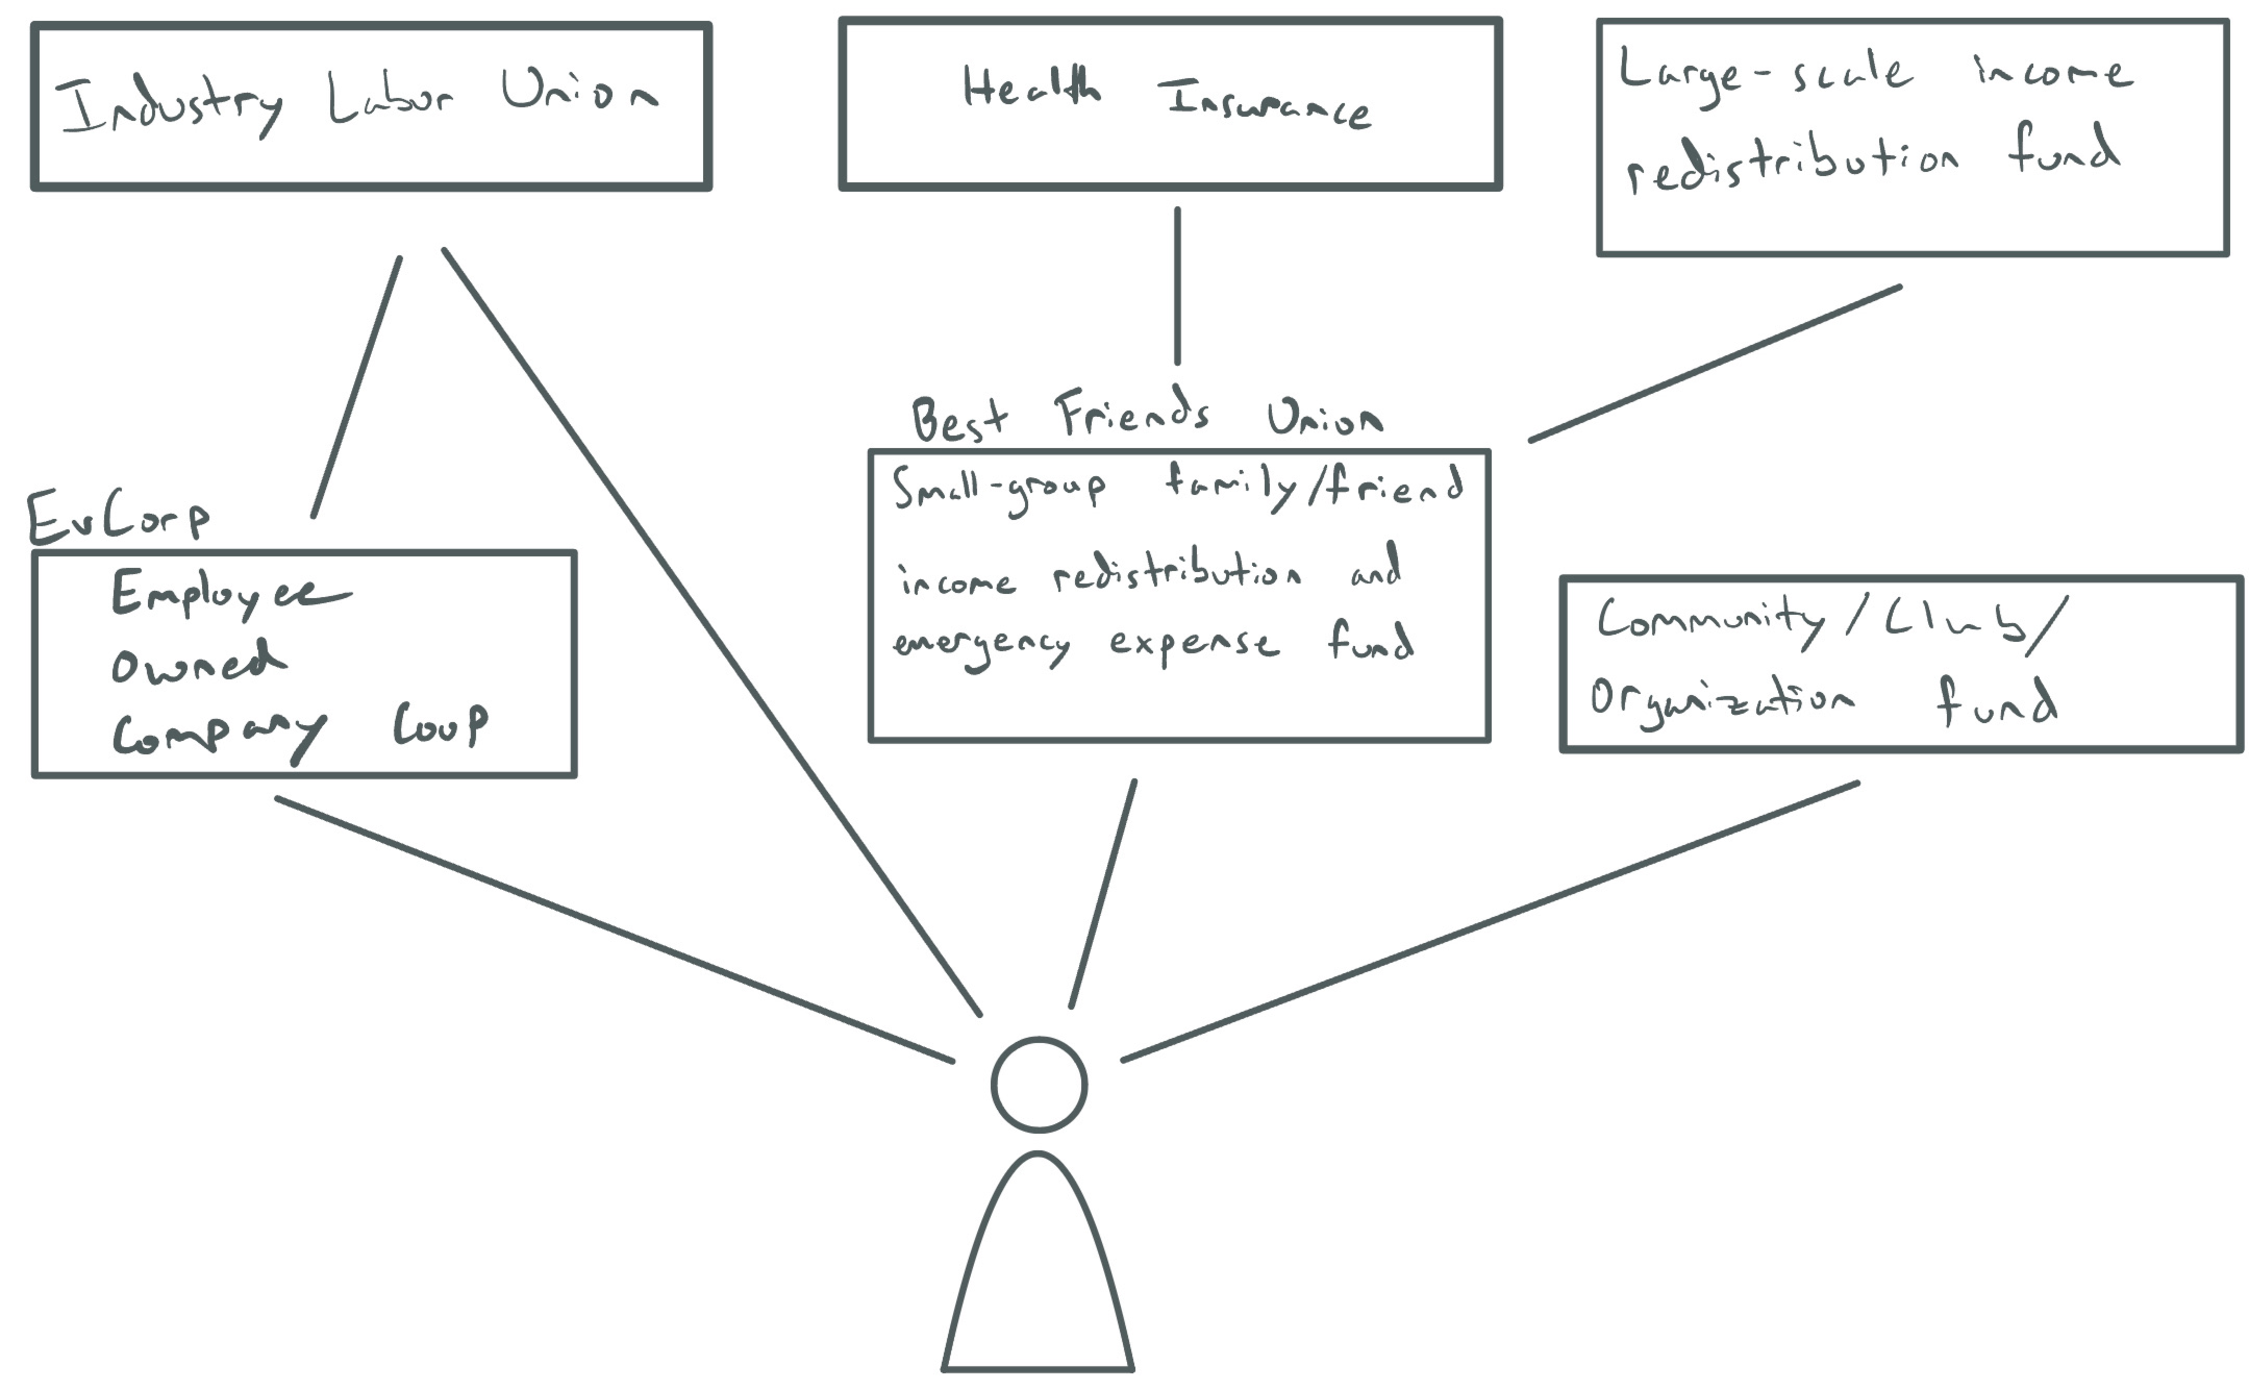
\includegraphics[width=\textwidth]{figures/IMG_1537E0469B4D-1.pdf}
    \caption{\textcolor{red}{need to remove community fund or write a paragraph about it}}
    \label{fig:person_in_groups}
\end{figure}

Going from closest to furthest connections, and then from left to right, first we have EvCorp, a partially-employee-owned organization with the goal of profiting from the creative potential of innovative people. 
Next, EvCorp might be situated within the context of a larger, potentially more decentralized organization such as a labor union.
The need for labor unions varies by industry, but an example of one that EvCorp might be affiliated with would be that of a teachers' union.
Alternatively, maybe an innovator invents a device that needs special training in order to be produced.
The people we hire and train to produce said invention would not be able to transfer these skills since we are the only producers.
This gives us an unfair sway over the market for this type of skilled labor, and would create incentive to unionize if we took advantage of that market power.
The real lesson here is does not concern labor unions, but the fact that many types of groups beyond those already described in detail may have some potential to exist in SECC version.\par 

Next up we have Best Friends Union, which has already been described as a financial tie between a small number of members that involves sharing income and expenses in order to mitigate individual financial risk.
This coalition might be nested within two other SECCs, the examples here being a health insurance DAO and another group with a similar design and purpose to Best Friends Union, but at a larger scale. \par

Motivation for participating in the first should be clear since the benefits of decentralized health insurance have already been described in Section \ref{section:Background}.
As to the question of why Best Friends Union would be shopping for health insurance collectively rather than each member shopping individually, the first answer should be why not?
After all, everyone's finances are already combined anyways, so it would be easier to send one monthly payment from the joint account of BFU.
The health insurance SECC would also prefer this for the same reasons that health insurance companies prefer to sign on companies: the process is less involved when you can do many people at once, and signing on groups diversifies risk.
If one member of BFU loses their source of income, the health insurance SECC doesn't have to worry because their friends will need to make the payments in their stead. \par

Finally, there's the large-scale income redistribution fund.
At first this may sound worthy of a pretty lengthy discussion, but in reality its explanation amounts to the same thing: diversifying risk.
Imagine that since Best Friends Union was started by me, an economist, and people tend to socialize with those similar to themselves, that all four of my friends are also economists.
This means that on our own, BFU is seriously vulnerable to a downturn in our field.
Wouldn't it be great if we could team up with a few other unions in order to diversify our risk?
Having people in the large-scale income redistribution fund that work in big tech, government, the trades, or the arts would prove very beneficial for us.
You might be thinking that people making programmer salaries would never want to split their income evenly with that of struggling singers, but keep in mind that SECC's are flexible, so the specifics of each one can vary greatly.
Maybe this large-scale income redistribution fund doesn't split everyone's income evenly, but instead according to a predefined acceptable level of inequality where programmers get to keep their fat salaries.\par




\subsection{Sub-settable DAOs}
\label{subsection:subset}

\textcolor{red}{Sources with stuff I have to incorporate}
\textcolor{red}{\begin{itemize}
    \item \fullcite{DAOstack}
    \begin{itemize}
        \item Talk about holographic consensus / genesis protocol as a method of scaling votes in large DAOs: \\ \fullcite{holographicConsensus1}\\
        \fullcite{holographicConsensus2}
        \begin{itemize}
            \item similar but likely not useful:\\
            \fullcite{predictionMarketsContentCuration}
        \end{itemize}
        \item \textbf{Ok so my sub-settable idea has already been done.
        And with a cooler name at that.
        Gonna need to at least delete this sectionif not massive rewrited to the whole thing}\\
        \fullcite{DAOstackWhitePaper}
    \end{itemize}
    \item 
\end{itemize}}

Decentralized Autonomous Organizations ("DAOs") are just a specific type of smart contract, and rather than inventing a fundamentally new capability for DAOs, here we are beginning to outline the definition of SECCs as a new type of DAO.
Currently, the code for each DAO is usually written with only that DAO in mind, and inter-organizational ("DAO2DAO") relationships are but an after-thought.
As such, any DAO2DAO relationships require individualized smart contracts to be written which detail the terms of the agreement.\footnote{
    \textcolor{red}{source maybe?}}
Leaving DAO2DAO interaction as an after-thought makes it heavily time and resource consuming to implement.
This inevitably discourages the creation of said relationships, so DAOs would benefit from a standardized framework for these interactions to exist within.\par 

In this Subsection, we define the "Sub-settable" part of the acronym as a standard framework for DAO2DAO interactions.
In it one SECC can join another SECC as a Member.
Notice the purposeful use of the proper noun "Member," which we define here as either an individual person or an entire SECC.
All SECCs have Members, each of which could be either a person or a SECC, and any SECC no matter how far up the ladder can join other SECCs as a Member.
The foundation is still comprised of individuals, but it's just SECCs all the way up.
In this way we no longer think of SECCs as categorically different from individuals, but just as scaled up versions; collective consciousnesses if you will. \par

Whether a given Member is an individual or a group, they will not be treated in a categorically different manner. 
The only differences will be that their contributions and responsibilities scale according to their size.
For example, if monthly payments for the health insurance SECC shown in Figure \ref{fig:person_in_groups} are \textcent$1$ (one unit of unspecified cryptocurrency) for an individual Member, then dues would be \textcent$5$ for the Member that is Best Friends Union, itself a group of five individuals.\footnote{
    In some cases it may make sense to implement slightly different rules for members that are groups, such as group discounts. 
    However, these discrepancies in the treatment of groups versus individuals should still function as a matter of scale, and not one of categorical difference.
    Meaning, in this case, that a transparent discount as a function $f(x)$ of number of individuals in the group $x$ with the following characteristics as example might be applied equally to all Members.
    \[f(1) = \textnormal{\textcent} 1 \]  
    \[\textnormal{as } x \rightarrow \infty \textnormal{, } f \rightarrow \alpha \textnormal{ where } 0 < \alpha < 1\] 
    \[f(x) \textnormal{ is monotonically decreasing on }[1,\infty)\]}
The important thing to note here is that each of the five individuals directly pay BFU which then pumps that money on through as one combined payment rather than each individual paying the health insurance SECC directly. \par

Similarly, if an individual in BFU needs to make a health insurance claim, then all five would vote to send that claim on up and later collectively share the responsibility of distributing the payout to the correct member upon receipt.\footnote{ \label{note:groupDiscount}
    Voting methods need not be simple democracy, and can be fit to the circumstances of the SECC, just as can be done in DAOs.
    For example, a popular DAO voting system is one where individuals can propose one of a predefined set of actions, and those actions are approved by default unless an objection is raised, in which case an actual vote is triggered. \\
    \indent \indent \textcolor{red}{*source*}}
In this way, SECCs acting as Members function identically to how a Member that is an individual functions, but at the scale of their group size.
"[T]he scale of their group size" means that actions of the sub-SECC are performed as if by consensus from the point of view of the umbrella-SECC, and their effect size is tied to the number of individuals in the sub-SECC.
For example, if the health insurance SECC was holding a vote, then an individual Member would get one vote while Best Friends Union would get the equivalent five, one for each individual, but the five could not be split.\footnote{
    This is similar to the Electoral College System in the United States, where the winner of the majority vote in the State takes the entirety of the State's assigned electorates.\\
    \indent \indent \textcolor{red}{*source*}} \par

Why might this be a helpful structure for DAOs to adopt?
Think of it from the point of view of the health insurance DAO.
Their main fear would be of an individual attempting to join and take advantage of the system by submitting a fraudulent claim.
If instead it is groups of people that are joining your health insurance SECC, and each of these sub-SECCs 1) contains individuals which know each other better than any two random individuals in the umbrella-SECC would, 2) has their sub-SECC's reputation within the umbrella-SECC at stake and 3) has to vote in order to allow the individual's claim to pass through, then this social dynamic should act as a filter against fraud. 
Why would you let your friend commit fraud when you know it creates the potential for BFU to be kicked out, thereby putting you at risk of losing your health insurance?
This type of sub-group responsibility dynamic is very useful for large DAOs that might otherwise consist of a crowd of anonymous individuals with no reason to trust each other outside of the incentives that blockchain smart contracts can directly provide.\footnote{
    One might ask, well why would this health insurance SECC ever choose to admit an individual as a Member?
    The answer is that they might not; current Members can decide/vote on who to admit.
    To say that SECCs are to treat all Members the same at the scale of their size once admitted into the collective, whether that Member be an individual or group, is not to say that SECCs are being forced to allow in both types of Members.}
Thus, a whole new world of potential for off-chain collaboration and trust is uncovered.\par

\begin{figure}[! ht]
    \centering
    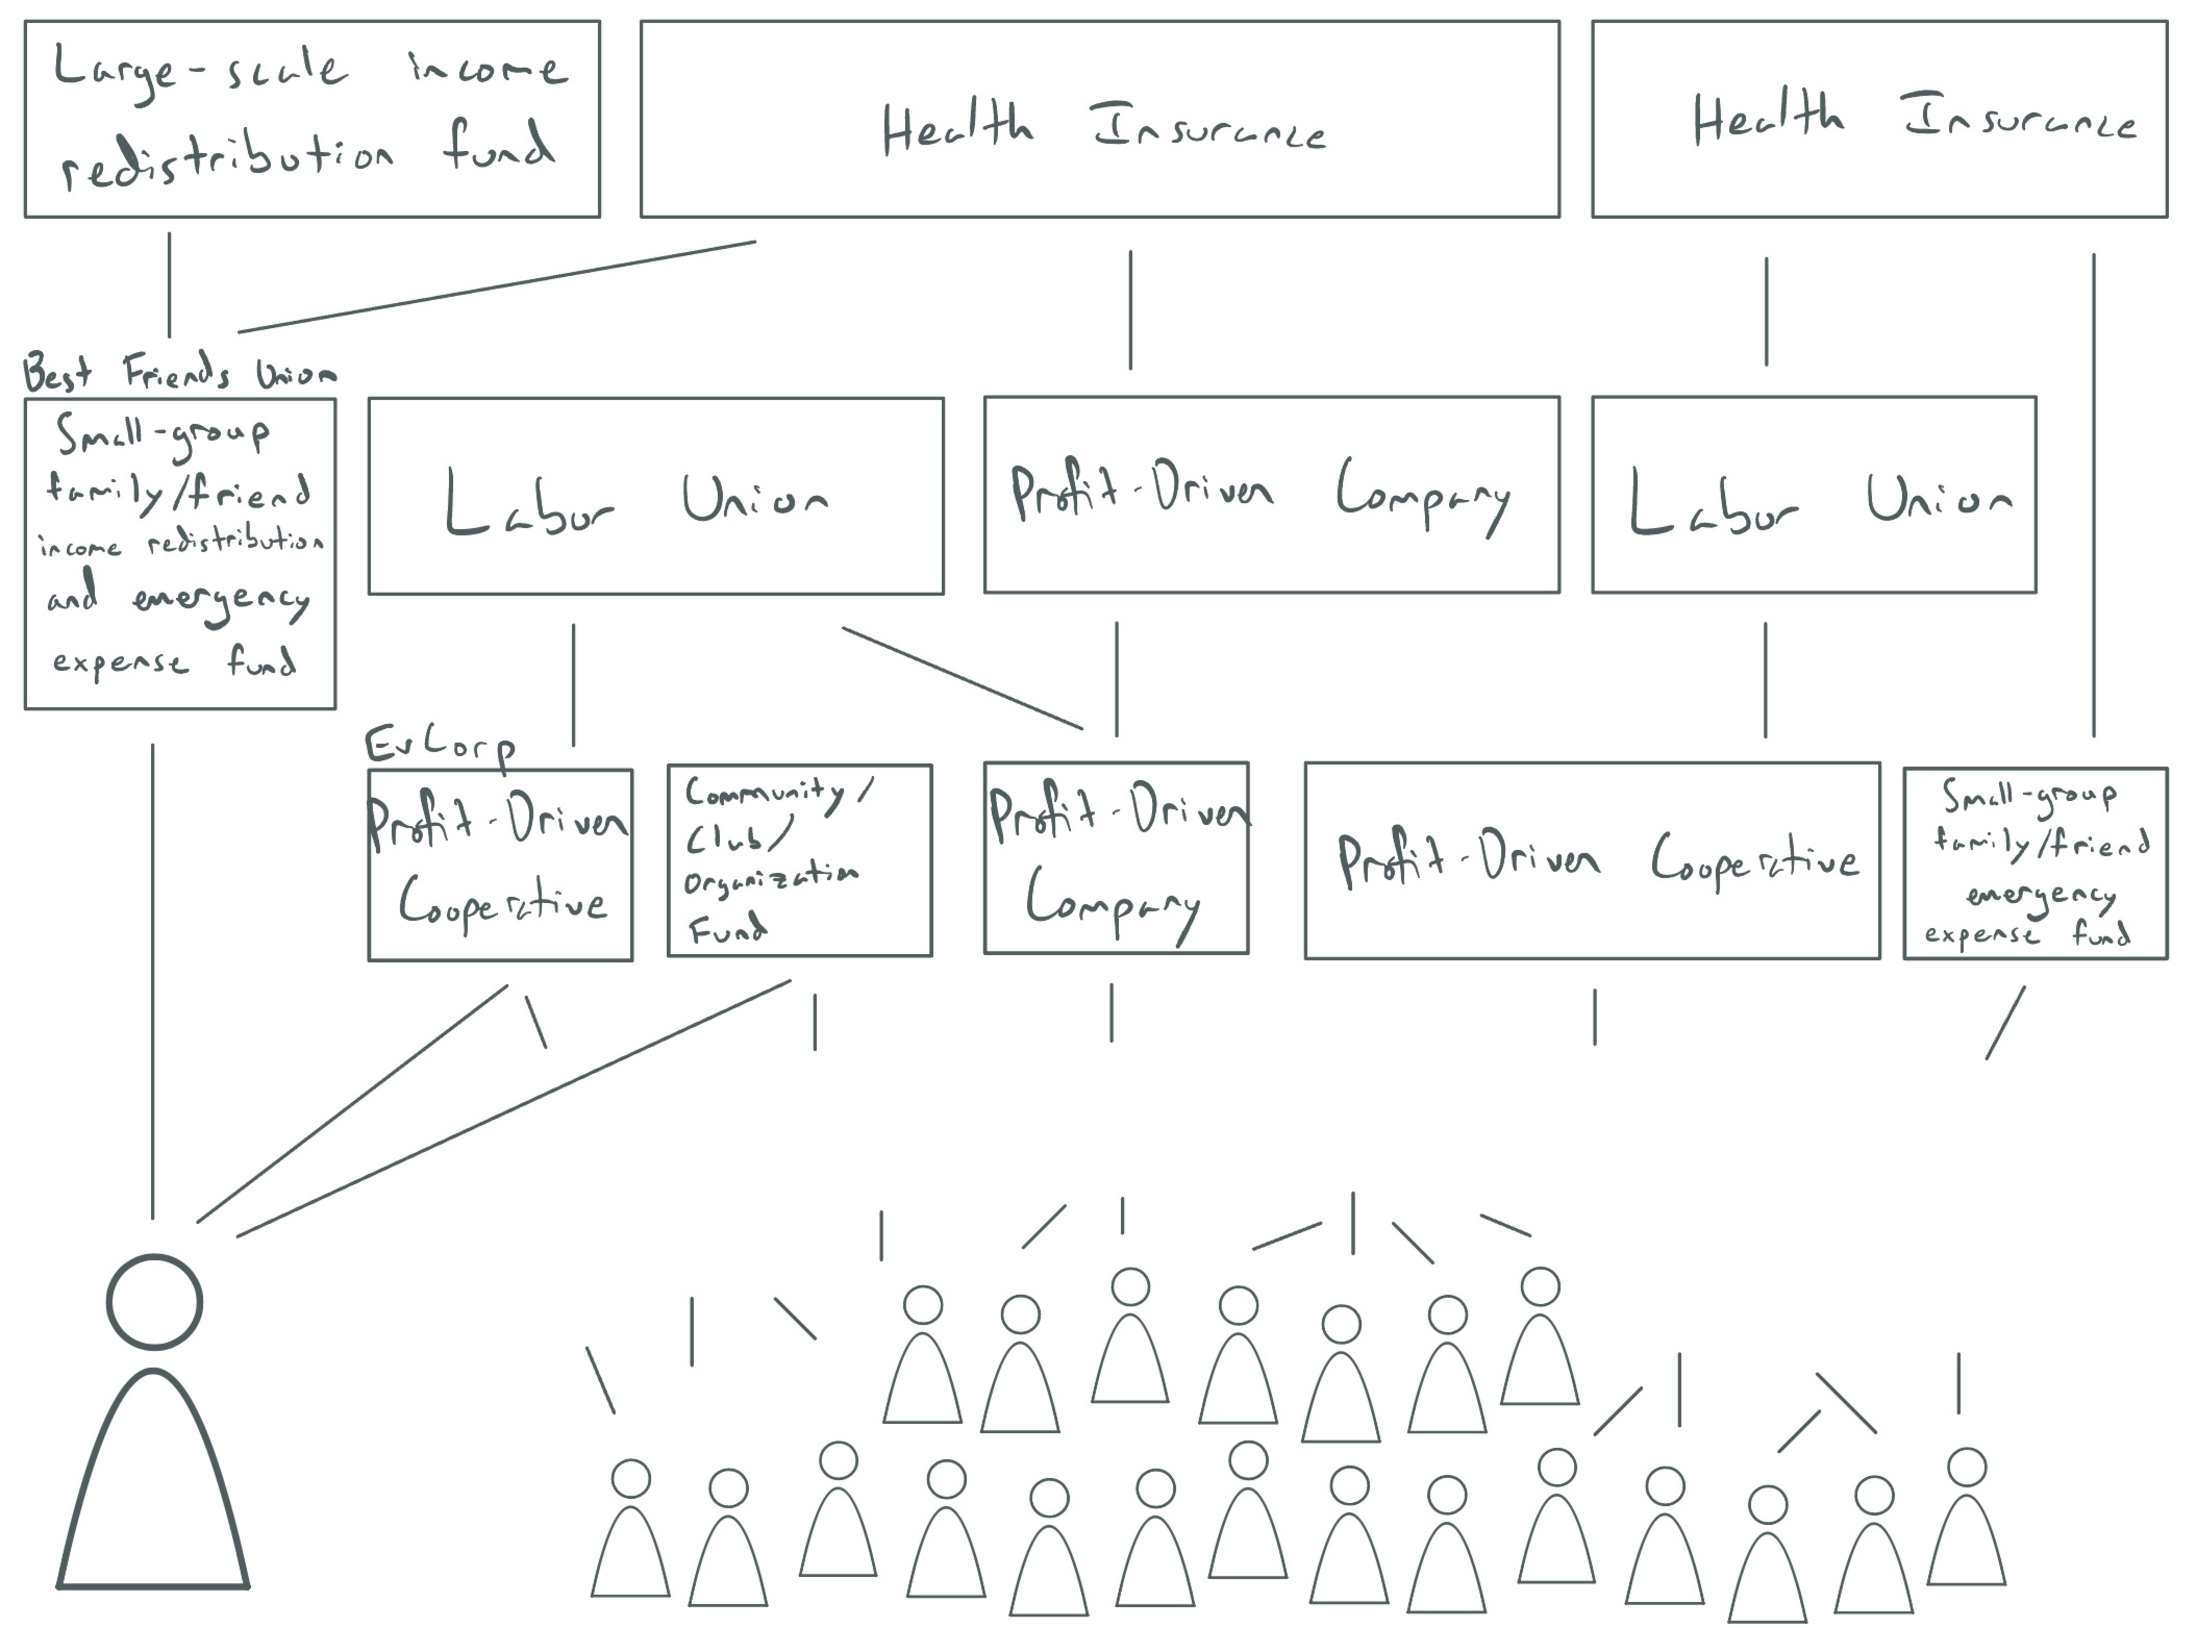
\includegraphics[width=\textwidth]{figures/IMG_B0CE257AF90D-1.pdf}
    \caption{Caption}
    \label{fig:modular_groups}
\end{figure}

This structure is also helpful for an individual nested inside multiple levels of SECCs.
Rather than fully participating in direct democracy to determine every single group action, a common strategy among DAOs is to do what is called \_\_\_\_\_ voting.\footnote{
    \textcolor{red}{figure out where i heard of this voting system and what it's called}}
In this system, proposals are enacted by default, with actual group votes only being triggered if an individual actively disputes the proposal.
This is beneficial for productivity because it prevents the group from being bogged down by every decision that needs to be made, as often happens in direct democracy.
Making DAOs sub-settable and using Members instead of individuals further enhances this decision making system.
Let us imagine a potentially fraudulent claim is spotted by a Member of the health insurance SECC, and they dispute the proposal.
Under the \_\_\_\_\_ voting system as it stands today, a significant portion of a non-sub-settable DAO's members must act to investigate the claim and come to a decision.
For SECCs however, the number of individuals needed to participate is drastically reduced, because each sub-SECC is its own Member that implements its own \_\_\_\_\_ voting system.
What this means is that rather than all five or even a majority of the individuals in BFU needing to participate, one individual can gather the information, make a decision, and propose a motion to have BFU vote a certain way in the umbrella-SECC's ballot.
If the other four individuals trust this active participant, then all five of BFU's votes will automatically be allocated according to the motion without the need to put time and energy into bringing every individual up to speed and voting.
If on the other hand one individual thinks it necessary, then the motion to vote a certain way can be disputed and BFU can initiate an election to determine how to allocate their collective five votes in the health insurance matter.\footnote{
    Through these two paragraphs I have drawn a parallel to the Electoral College System in the United States by describing a winner-takes-all effect because I believe it to lead to a more concise explanation of the general idea.
    However, other than keeping with this "Individuals and SECCs are treated the same except in respect to the scale of their group size" story, there is no actually reason why at this point the votes from Best Friends Union could not be split.
    There would be no actual issue if the directly democratic votes were sent up the chain, say for example four in favor and one against.\par
    The result of this edit would in fact parallel that of eliminating the Electoral College System in the United States.
    With the winner-takes-all design, individuals will more often defer to the attentive individual's proposed motion and spend less time participating themselves, because they know that in order to change anything they would have to convince a majority of their small group.
    From an "everybody should vote" perspective, this is a bad thing, but in terms of efficiency, the effect likely saves massive amounts in exchange for the relatively infrequent case of an election result that would have played out differently in a direct democracy.
    This efficiency improvement should not be taken lightly, since it could have a large effect on the manageability of governing the SECC and therefore the feasibility of SECCs in general. 
    Also, it is important not to point to U.S. presidential elections to get an idea on the frequency of this negative effect, because the Electoral College System has the additional major flaw of actually giving some citizens (low population density states) more voting power than others (high population density states).}\par

In this way, SECCs allow for a structure similar to that of representative government, but without the possibility of those pesky politicians sticking around past their term.
By allowing for fluid and case-by-case movement between direct democracy and representational forms of government, SECCs will allow a given voting body to take advantage of all of the benefits and none of the encumbrances of either voting system.
To bring the government analogy further, the case of one Member within an umbrella-SECC proposing a motion and it passing without dispute would be akin to the efficiency of an oligarchy or monarchy, depending on whether the Member is a SECC or an individual, respectively.
In this way, the Sub-settable structure combined with the \_\_\_\_\_ voting system actually allows for on-demand fluidity between all forms of governance, all the way from democracy, with its priority on the people's interest, to monarchy, with its advantages in implementing quick decisive action.\footnote{
    It is not lost on me that there has already been discourse about using DAOs to replace some or even all functions of government, and that the structure laid out here could play a part in such a blockchain government.
    Just imagine the complicated but fluid and efficient voting structure that would result from BFU being a sub-SECC to a local political party, which is then a subset of a regional SECC, which is itself a subset of a national decentralized political party SECC.}\par







\subsection{DAOs As Clusters}
\label{subsection:clusters}

\textcolor{red}{\begin{itemize}
    \item variance in how rigid vs dynamic the groups are
    \item display of how clusters can pop off from EvCorp that looks like molecules bonding to each other
    \item in the current space, DAOs are complicated smart contracts made for fulfilling a specific purpose. It is only after the fact that DAO2DAO communication is considered. My point is I want an open source framework / code-base for all these DAOs to build on top of that establishes standard structures for communication, money, and incentives to travel along. And I want these standards to be flexible, essentially abandoning our current idea of static companies and amorphous decentralized organizations in favor of these more loose "clusters" with varying degrees of interconnectedness.
\end{itemize}}



\begin{quote}
    \textit{Author's Note:}\\
    \textit{In this subsection we will be using the word "individual" rather than the proper noun "Member" defined in Subsection \ref{subsection:subset}.
    This is entirely because I believe thinking about this concept in the familiar context of individuals working together in a company will be helpful with comprehension on a first pass of the idea.
    In reality this substitution is not a technical claim, so the entire Subsection could be reread a second time using the proper term.
    Such a substitution would entail a merging of the "Subsettable" concept with the "Clusters" concept in a manner that will likely lead to a whole that is greater than the sum of its parts.
    This synergy is to be referred to as "Enmeshment" and will be discussed later in Subsection \ref{subsubsection:enmeshment1}.}\par
\end{quote}

%\vspace{0.2in}

Now that we've defined the "Subsettable" part, and since the "Cooperative" word was already described in Subsection \ref{subsection:cooperative}, we can move on to the "Clusters" piece of the SECC acronym. 
When thinking about relationships between individuals within an on-chain organization, there are multiple questions which the motivate the idea to come.
How might organizations restricted to the blockchain be able to efficiently interact with the off-chain real world?
Can incentive structures be designed to reliably incorporate off-chain sources of revenue?
What is the optimal number of individuals to comprise a group?
By what means can we reach this ideal number, which may be group-specific and therefore need to be defined on a case-by-case basis?
Under what conditions would an individual be motivated to join or leave a group?
What do these entry and exit processes involve?
How can we design these incentives and processes to ensure that groups reach their ideal membership size?
Might an individual feel locked into a given Subsettable Organization if it is a sub-SECC of another more important umbrella-SECC?\footnote{
    For example, Best Friends Union is a subset of a health insurance SECC, and one would not want their exit from BFU to necessarily and fully terminate their health insurance. 
    This would effectively trap the individual by making it against their best interest to leave the sub-SECC.} \par 

Enter organizationss as "Clusters," which we define as groupss with sources of incoming revenue where each individual's role and membership is dynamically defined and mapped by connections involving 1) revenue that cascades out from those with direct access to a revenue stream and 2) incentive structures coming both top-down from the revenue stream holder(s) and horizontally from other individuals attached to the same revenue stream. 
The goal here is to merge on-chain activity, decision making processes, and incentive structures with that of off-chain real-life businesses.\par

Take for example the first individual with a revenue stream, myself, the founder of and first holder of the "Innovator" position at EvCorp.
Presumably when starting this business I have enough money to fund it in the short term.
By trading in my government money for cryptocurrency, I will be creating the first Revenue Stream Node ("RSN"). 
From here I will be designing a series of incentive structures that pay out cryptocurrency from my RSN to individuals upon their completion of work.
I personally prefer working with people that I know to some degree, even if just by zoom call.
As such, once I find employees, EvCorp's Revenue Stream Node will pay them an agreed upon amount every other Friday if I feel satisfied with their progress, or otherwise terminate the relationship.\par

As of yet, nothing about this structure has differed from what a traditional legal corporation is designed to do, except that my employees don't have the same benefits or protections under the law due to EvCorp's existence solely on the blockchain.
It is also the case that in a DAO this design would not be possible.
The structure I have detailed so far is centralized in that I, a single entity, maintain complete authority over EvCorp's goals, decision making, and distribution of rewards.
Many blockchain and DAO fanatics (henceforth "Crypto-Chads") will be put off by how this proposal is beginning and suggest that I instead go and start a corporation.
Again, the goal here is not decentralization for decentralization's sake, but rather to blur the lines between DAOs and traditional corporations by unifying on-chain and off-chain incentive structures.
It is important to remind decentralization-loving Crypto-Chads that top-down governance structures can have benefits as well, such as faster decision-making and the ability to enact concrete plans over the long term.\footnote{
    \textcolor{red}{footnote describing said benefits. Efficiency, decisiveness, taking counterintuitive approaches, focusing on long term goals, etc.}}\par

Anyways, at EvCorp I have a few ideas for how to get started. 
As described in Subsection \ref{subsection:EvCorp}, I'll want to begin with a teacher with a PhD in a subject I am curious about to help in my studies, maybe an assistant, and a software developer to run the website.\footnote{
    In reality, we might want multiple programmers, teachers, etc. but keeping each position in the singular will trim down on the writing and avoid unnecessary complications in the explanation. 
    For now, and for the developer especially, let us just give the person in each position god-like productivity powers when necessary.}
The programmer will become our second revenue stream once the website starts generating ad revenue.
In a traditional corporation, I as founder would own the website, so I would be within my rights to remove the developer's access, replace them with someone else, and sue them if they stole any of the company's intellectual property.
However, since EvCorp is just a Cluster Organization with no legal ownership of each individual's work, the programmer has full control of a new revenue stream.
They may decide to do with the money what they like, whether that be to boost their own income or to establish their position in EvCorp as a new RSN.\par

You might be wondering how I control my newly powerful employee.
Well, I might not; the programmer has free will, incentives that could conflict with my goals, and no leash around their neck.
If they decide that the resources in their direct control are profitable enough on their own, then they have the option of splitting off and starting their own business.
In this sense, EvCorp is directly defined as whatever individuals receive funding from and therefore work towards the goals of my RSN.
However, the money streaming from my RSN may still be enough to keep the developer working with me.
Furthermore, a split from EvCorp would leave the programmer without access to the teacher who has been making the videos that bring in the ad revenue.
Unless said income is lucrative enough to steal the teacher away from me, then I now have a second bargaining chip.
In exchange for me funding the teacher and potentially directly paying the website developer some amount as well, I will still maintain influence over how our website is run.
At any point in the future, the deal may have to be edited depending on the changing power dynamics between our RSNs.
Maybe eventually the programmer brings in so much ad revenue that they can even steal the teacher away from me.\par

Now suddenly EvCorp consists of two RSNs with pay structures feeding down to the non-RSN employees that adjust dynamically based on how each owner thinks they can best optimize their own revenue stream.
At any given time, does one RSN send money to influence the other, or do they act as separate entities?
For visual depictions of each scenario, see Figure \ref{fig:clusterInteraction}.
The first case was described in the previous paragraph.
The second involves neither EvCorp nor the programmer's RSN seeing any benefit in extorting influence over one another, but they do happen to share employees.
Each shared employee might experience different ratios of pay from the two, while others will only be paid by one RSN or the other.
For example, the teacher could split their time between the two according to who pays most, while my assistant would be entirely EvCorp funded.\footnote{
    \textcolor{red}{in some footnote I need to define a model of two RSNs competing for a single employee's time and how that results in a larger percent of profit going towards labor. 
    Contract workers that take gigs from multiple companies already take advantage of this effect (so maybe I can co-opt some research about them) but this brings that dynamic to all employees of single companies.
    Not sure if that model should go in this footnote or one that shows up later}}\par



\begin{figure}[! ht]
    \centering

    \begin{tabular}{c|c}
        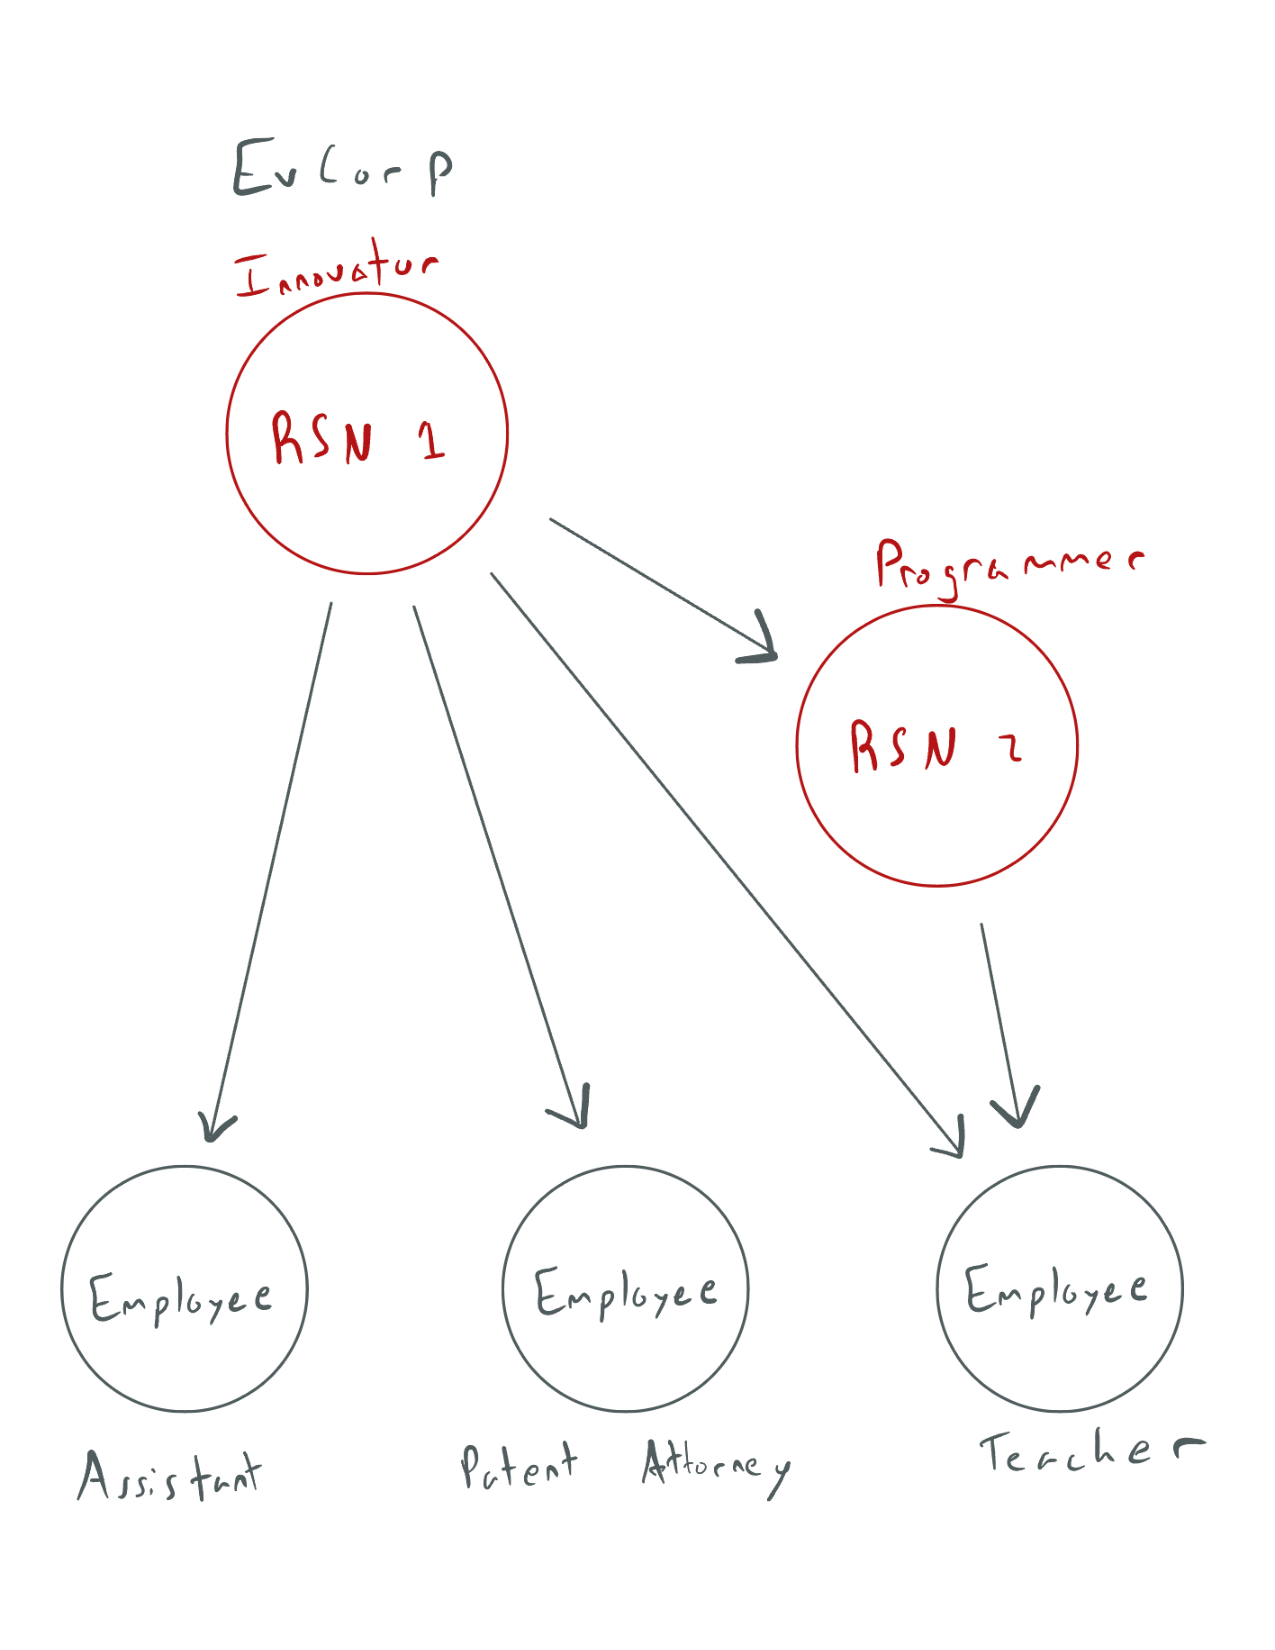
\includegraphics[width=0.5\textwidth]{figures/IMG_38A57C8FE8C1-1.jpeg.pdf} & 
        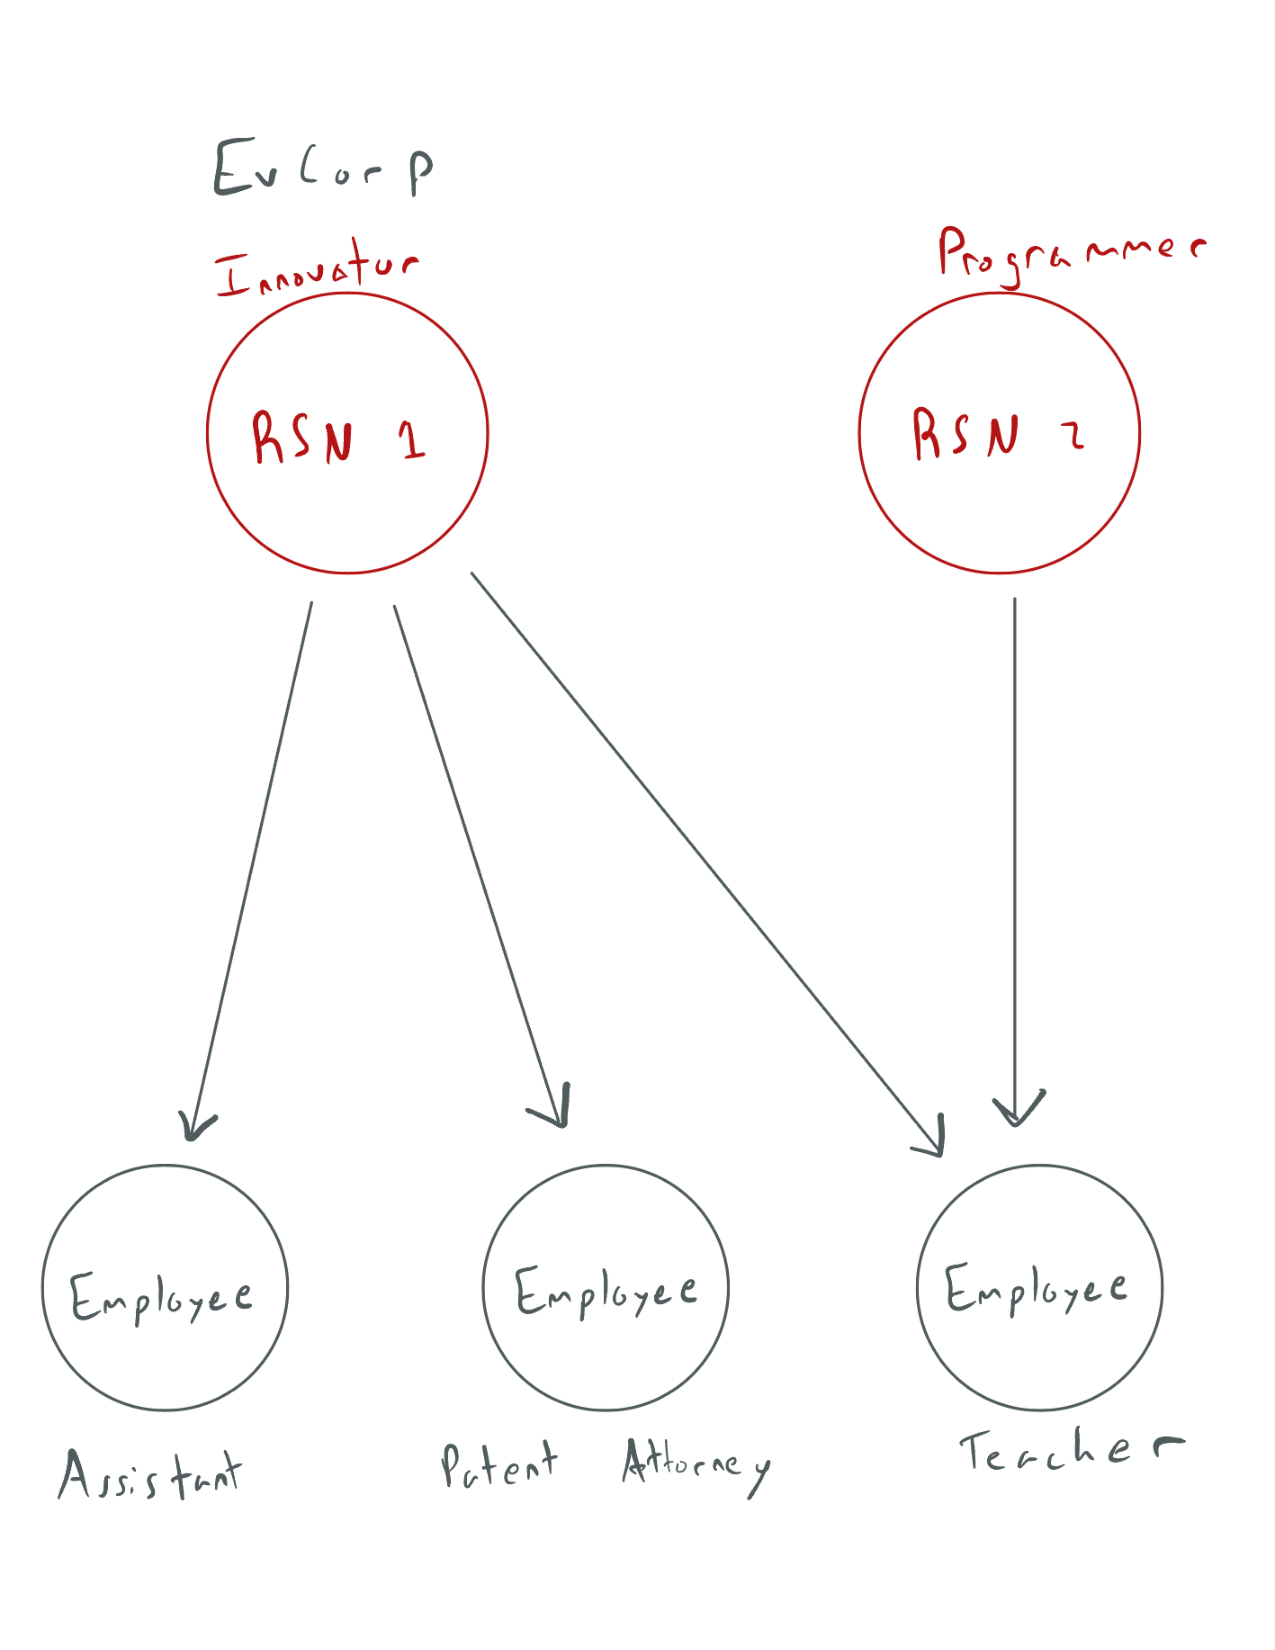
\includegraphics[width=0.5\textwidth]{figures/IMG_C8BDE58C72C5-1.jpeg.pdf}\\
    \end{tabular}
    
    \caption{caption}
    \label{fig:clusterInteraction}
\end{figure}


Finally, we are ready to strictly define the title term of this Subsection.
A "Cluster" consists of at least one RSN paying at least one individual for their labor, whether that work be verified by on-chain decentralized means or through the off-chain real-life interaction of the individuals involved.\footnote{
     On-chain decentralized means of employment can use the same incentive and verification structures already implemented in traditional smart contracts and DAOs.
     Off-chain labor can be verified just as is done by traditional legal corporations, meaning a manager (the RSN owner) either witnesses their employees' labor in person or, in the case of a remote worker, waits to receive work product before verifying satisfactory performance.}
Further components to the definition of a Cluster Organization are as follows:
\begin{itemize}
    \item Two RSNs are deemed to be part of one single Cluster if one RSN, the "payer," partially funds another, the "payee," in order to incentivize the latter to help work towards the goals of the former.
    
    \item For chains of three or more RSNs, the one not receiving funding from any other is referred to as "central."
    Those receiving funds directly from the central RSN are deemed "first peripheral," while those receiving funds directly from a first peripheral RSN are deemed "second peripheral," and so on.
    These can be referred to in aggregate as "peripheral RSNs."
    
    \item A cluster is referred to according to the name of its central RSN.
    
    \item When one RSN directly funds two or more peripherals, the chain of peripheral RSNs is said to be "branched," creating "siblings." 
    However, that is as far as the use of familial terms should go, because RSNs need not send money down the line linearly.
    
    \item An RSN might choose to funnel money horizontally to another at the same peripheral order as well as upwards to an RSN of higher peripheral order.
    However, this higher order payee should be outside of the direct line between the payer and the central RSN. See Figure \ref{fig:funnelUp}.
    
    \item Any given relationship must consist of at least one individual employee or peripheral RSN downstream of the central RSN in order to be considered a Cluster, but a peripheral RSN need not necessarily hire any individual employees.
    
    \item Two or more RSNs, either within the same Cluster or in different Clusters, can fund a single employee.
    If an individual is funded by two or more RSNs from different Clusters, they are said to be employed by more than one Cluster.
    Because we are using Clusters rather than RSNs in our linguistic analogy to companies, one individual funded by two or more RSNs within the same Cluster is not said to have more than one source of employment.
    Rather, these cases should be thought of as analogous to an employee that does work for/with more than one department within a company.

    \item Although individual employees are not RSNs in that they do not bring in new money, they do in all other ways function the same as an RSN.
    This means that they can send money to other individual employees and even to RSNs.
    This money can travel down the chain, horizontally to other individuals or RSNs at the same peripheral order, and even up the chain as long as it is not going to an individual or RSN placed directly between themselves and the central RSN.
    The only thing differentiating individual employees from RSNs is the fact that RSNs have a source of off-chain or at least off-cluster revenue, whereas individual employees receive all their funding from others within their cluster.
    Now with this new definition of employees, it is more fitting to use the term "Labor Node" ("LN") because it better expresses their functional similarity to RSNs. See Figure \textcolor{red}{X} for a depiction of money streaming through LNs the way it does through RSNs.
\end{itemize}

\begin{figure}[!ht]
    \centering
    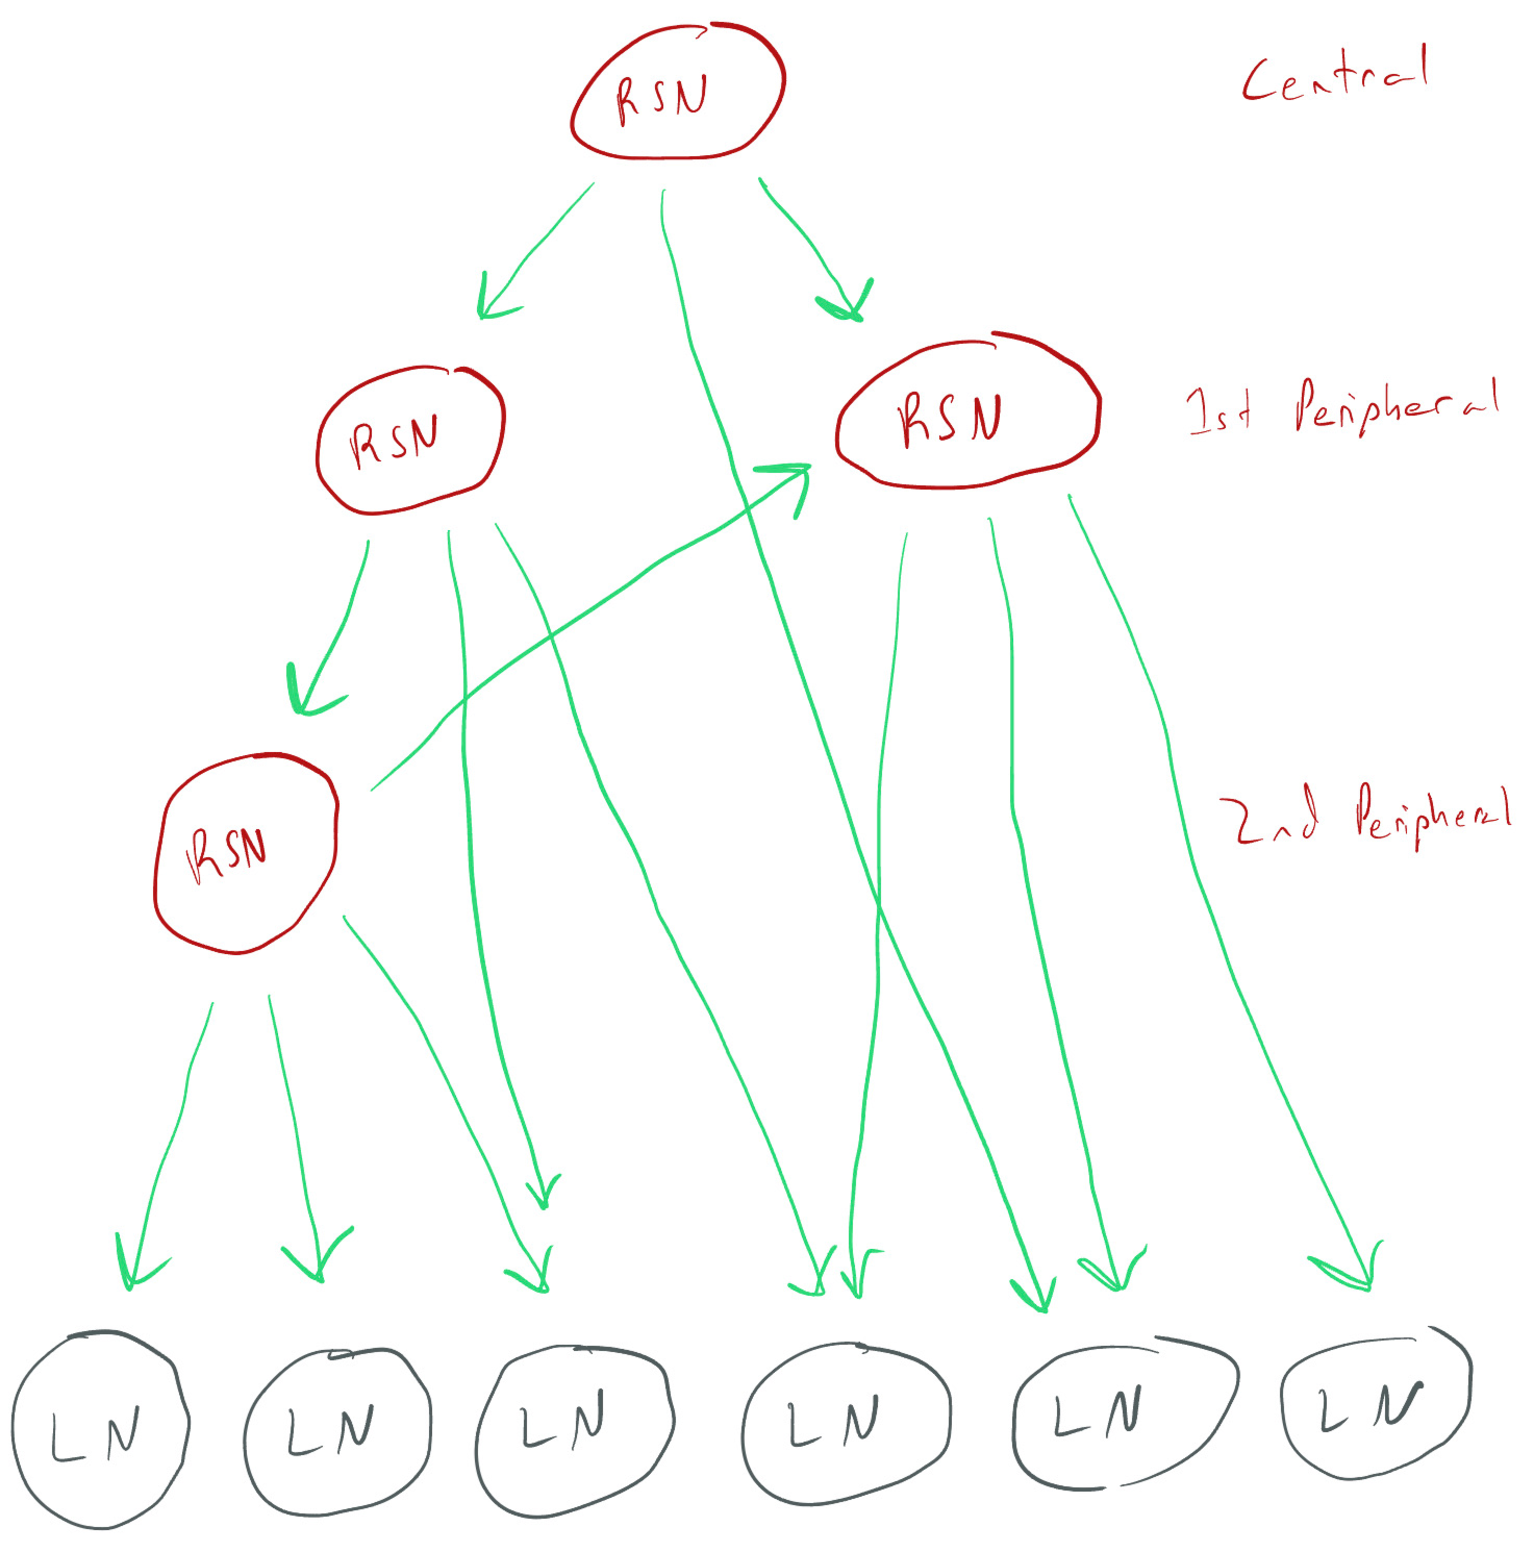
\includegraphics[width=\textwidth]{figures/IMG_680F7D487817-1.pdf}
    \caption{\textcolor{red}{need a diagram showing LN's as being able to pump money through each other as well}}
    \label{fig:funnelUp}
\end{figure}

Let us compare this new structure to that of traditional corporations.
In the latter all property, revenue streams, and liabilities are owned solely by the legal entity.
These companies have a top-down power structure with the CEO deciding how to allocate resources, tasks, and funding.
This necessarily means that decentralized economic information will not be accounted for, an issue that only gets worse as the company grows in size.
Decentralized economic information are those facts which can only be known at the detail of the individual employee or owner of a very small business.\autocite{hayek1945use}
When writing out the company budget, deciding how many employees to hire, and how to distribute the workload, there is no way the executives on the top floor could have an accurate idea of each employee's capacity.
This is obvious to anyone who has sat around the office with nothing to do, or struggled to meet an unrealistic deadline.\par

The top-down power structure makes traditional legal corporations inherently inefficient for the same reason that centrally planned economies are inefficient.
Centrally planned economies are those for which the government takes over the role of the free market system in deciding where to allocate resources.\footnote{
    \textcolor{red}{source}}
Rather than spend money at the supermarket for however much bread your family needs, the government gives you an amount of bread it predicts you will need.
The difference is that when a centrally planned economy fails an entire nation is destabilized, whereas when a corporation fails everyone just looks for a new job and a different company will peacefully fill the void.
It is through this trial and error process that entrepreneurs have been able to create wealth in aggregate for capitalist economies.
If anything, the inevitable failure of corporations (none last forever, and few more than \textcolor{red}{X} decades\footnote{
    \textcolor{red}{source}})
has acted as their only saving grace by creating a gambling arena that incentivizes entrepreneurs to subsidize the growth of capitalist economies with the money they put into failed ventures.\footnote{
    \textcolor{red}{cite taleb for providing this interpretation of the advantages of free-market economies}}
This failure-followed-by-replacement mechanism is analogous to the survival-of-the-fittest dynamic in evolution and acts to partially compensate for the inefficiencies of the currently commonplace top-down power structure in corporations.
Furthermore, it is through this same competitive dynamic that we should expect to eventually find a superior system to top-down control.
It is reasonable to praise capitalism for the increase in living standards it has created through its encouragement of specialization, this survival-of-the-fittest dynamic, and its partial incorporation of decentralized information, but to idolize the current commonplace company structure is akin to arguing that a given biological species has no more need to evolve.\par

In contrast, with clusters each resource, incoming revenue stream, and source of liability is owned and controlled by an individual.
Individuals within a cluster incentivize one another to work towards each others' goals through the simplest means available: paying each other the market price in exchange for their labor and access to their capital.\footnote{
    For the non-technical reader, capital is defined as "anything that confers value or benefit to its owners, such as a factory and its machinery, intellectual property like patents, or the financial assets of a business or an individual." In economics the two drivers of wealth are labor and capital, and in recent years capitalist economies have seen the share of income attributable to capital rise while that of labor has stagnated. This means that companies and those who own them have continued to get even richer, while the average person has fallen behind. Cluster organizations attempt to give ownership of capital back to the employees responsible for creating the capital in the first place, thereby diminishing wealth inequality.\\
    \indent \indent \fullcite{capitalDefinition}\\
    \indent \indent \textcolor{red}{source for share of income going to capital increasing since whatever decade. 
    Maybe both a solow model estimate and a reference to eric weinstein's discussion of its importance and the general fuckery that's been happening since whatever date}}
As such, all work is essentially brought into the gig economy.
Furthermore, just as prices have been used to quickly and efficiently communicate decentralized information in the consumer market, they can now finally do the same in the labor market.
For decades labor movements have rightfully fought against this occurring because supply and demand are not frequently kind to the common worker.
However, that is no longer the case now that 1) laborers can easily and more efficiently get benefits through Subsettable Organizations that have traditionally been attained through employers, such as group health insurance, 2) the source of money is now broken up between many revenue streams instead of a single decision maker, thereby increasing demand for labor since RSNs within a cluster (which are akin to team or department leaders within a corporation) must compete for an employee's work, and 3) ownership of capital has been partially redistributed from the capitalist to the workers.\par

In EvCorp, I have direct access to my bank account that I used to kickstart the venture, and presumably my research will eventually bear fruit with a money-making patent or business idea that can take over the job of funding my RSN.
I will likely hire an entrepreneur to run said venture rather than do it myself, and they will be able to create their own RSN once the business starts making money.
The programmer has direct access to the website that makes money off ad revenue, so they fully control what happens with that website and the money it generates.
They then create an RSN to pay out money to other employees in exchange for their labor, with the goal of further augmenting the revenues of the website.
As the online lectures and idea discussion forums attract users, they will eventually educate people who will then have their own money-making ideas.
Those people can create their own RSNs which may or may not join my cluster.
The lawyer will do all the boring lawyer-y things for whichever of these new ideas happen to be patentable, thereby generating revenue for themselves from legal fees and for the innovators from licensing royalties.\footnote{
    \textcolor{red}{footnote addressing concerns here with idea ownership and whatnot}}
The lawyer will create their own RSN which pays out the programmer's to have their ads put up on the website and encourage the creation of more patent-able ideas.
The teacher will be the Labor Node funded by both the programmer who posts video lectures and the innovators that want direct tutoring.
This structure comes together to create a symbiotic relationship between laborers,\footnotemark the owners of capital,\footnotemark and those that fit into both categories.\footnotemark \par
\footnotetext{The teacher and the lawyer.}
\footnotetext{The innovators.}
\footnotetext{The programmer and entrepreneur.}

In contrast, if I had started EvCorp as a legal company, then I would own the website, the teacher's video lectures, and the intellectual property of the innovators.
This traditional dynamic would open the possibility for me to pay them far below their true value since I come to own all the capital they create immediately upon its inception.
In this sense, the traditional market value for labor does not properly measure the downstream effect of capital created by labor, and therefore undervalues said labor.
For example, the programmer is significantly more valuable when they own and stay in control of their own website creation.
However, thanks to EvCorp's partially-decentralized ownership through split streams of revenue, I am forced to take into account the interests of at least every individual with their own RSN rather than just myself.
While this is not 100\% employee ownership since LNs, such as the teacher, still exist without their own revenue stream, I think it should be pretty clear that the perverse incentives of top-down structures have been mitigated by distributing power among many key individuals rather than a single parasitic owner. 

%\begin{figure}[!ht]
%    \centering
%    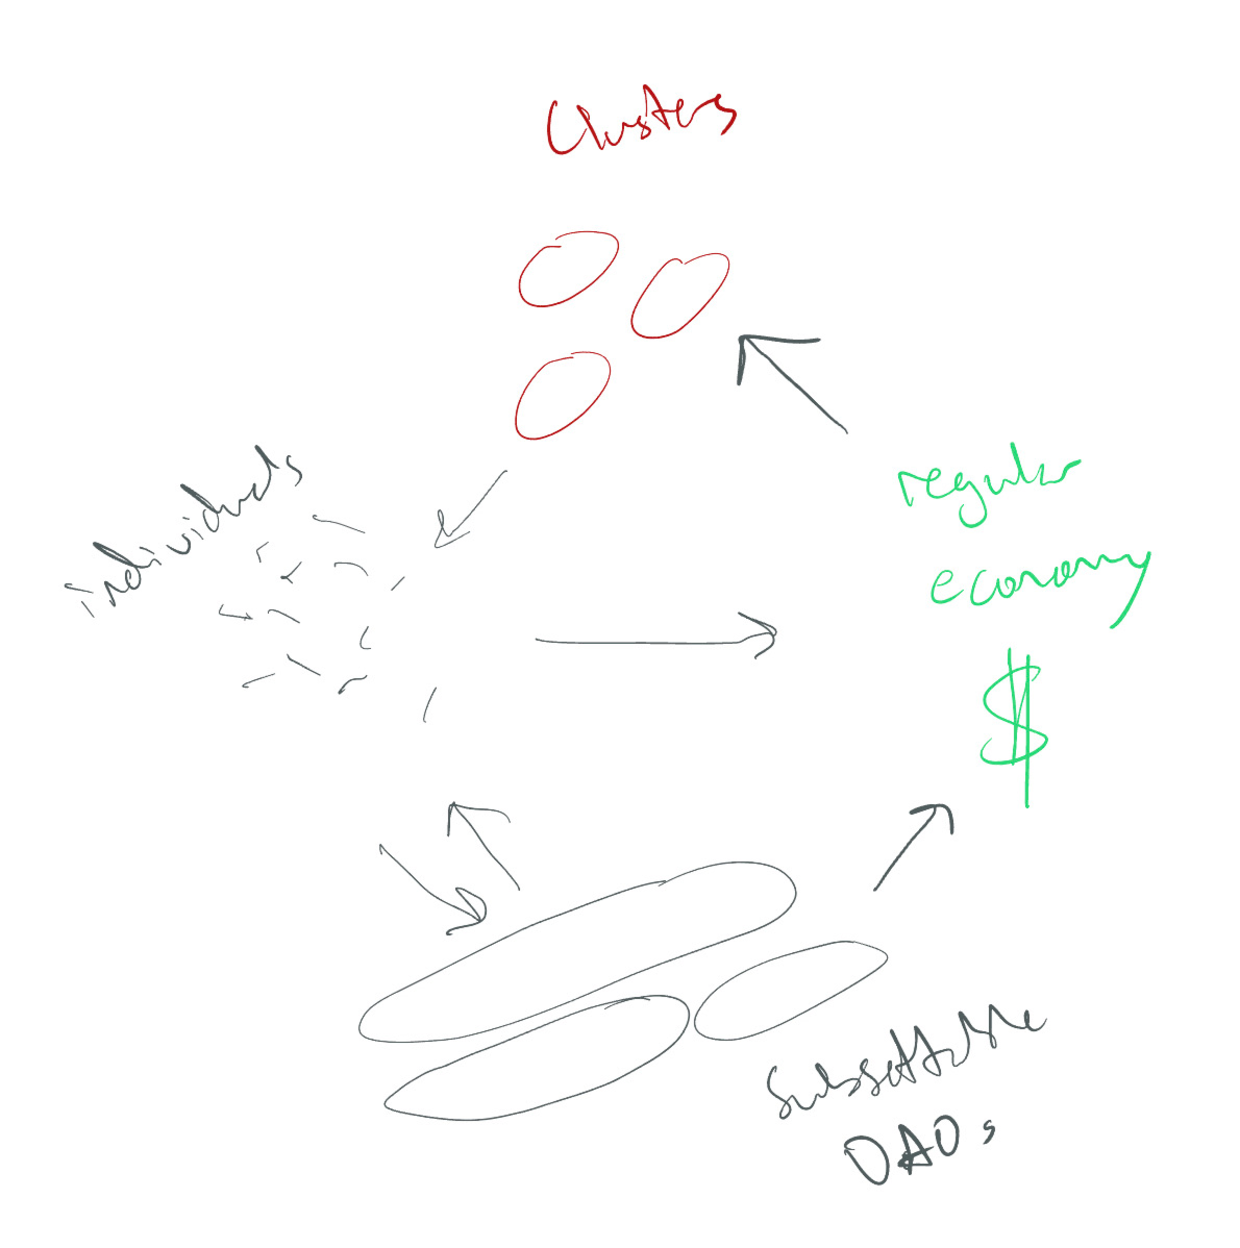
\includegraphics[width=\textwidth]{IMG_1012.pdf}
%    \caption{Caption}
%    \label{fig:economy}
%\end{figure}

%\begin{figure}[!ht]
%   \centering
%    \begin{tabular}{c}
%         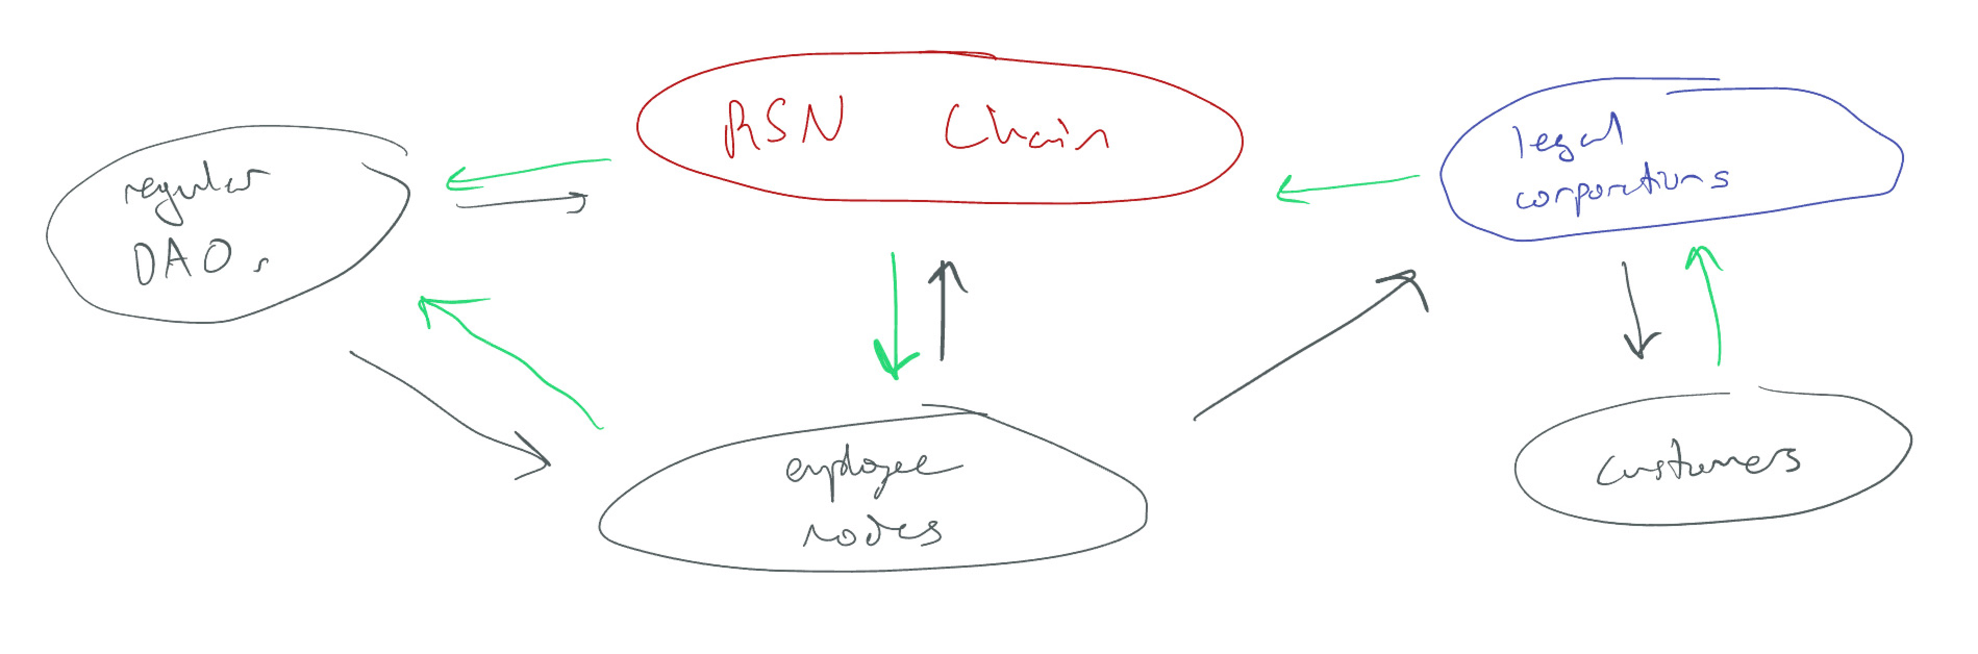
\includegraphics[width=\textwidth]{IMG_305A22D3211A-1.pdf} \\
%         \hline
%         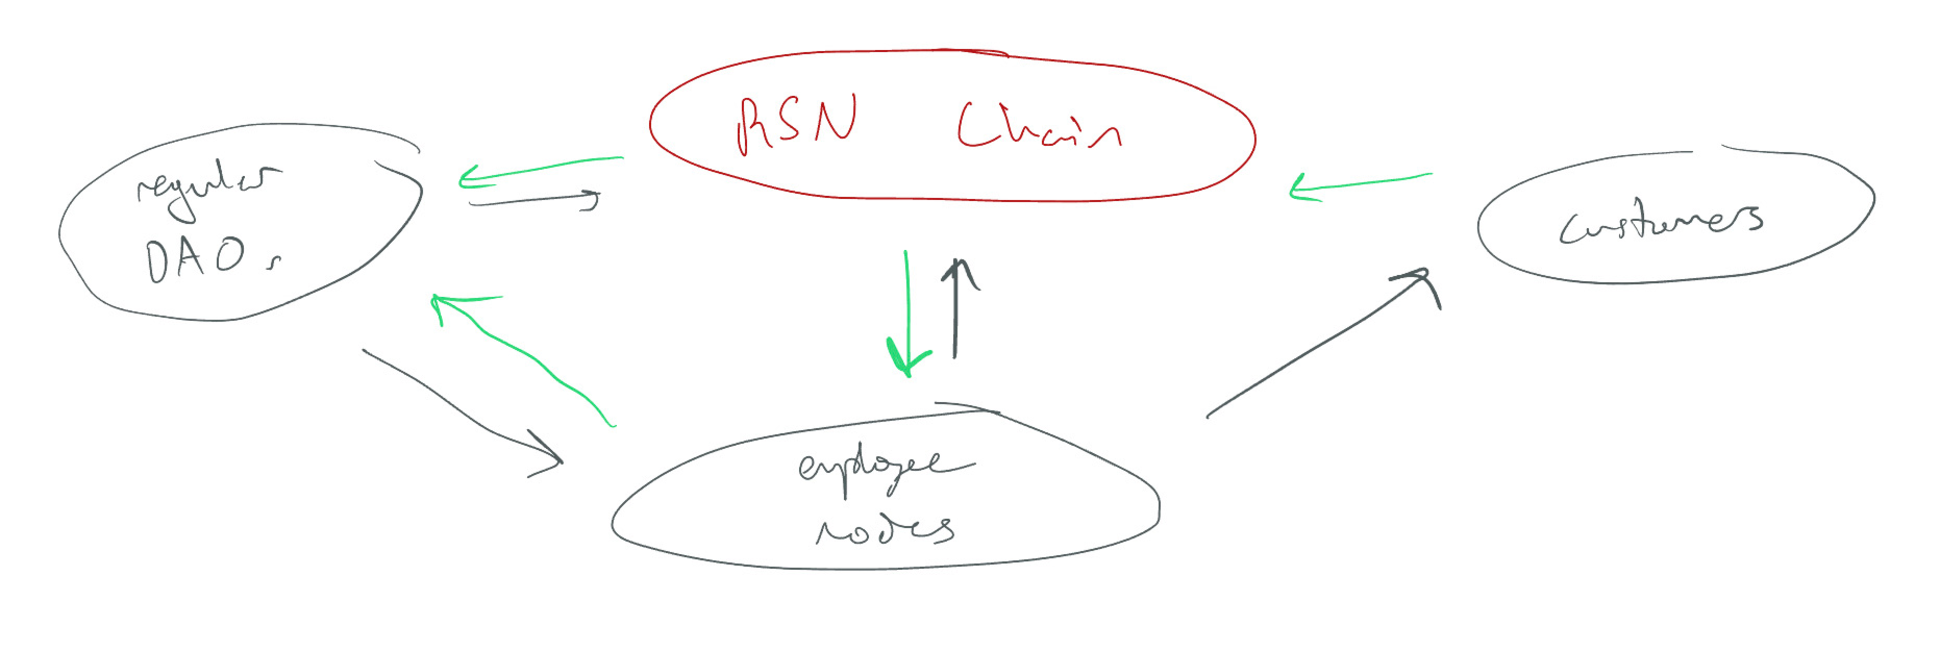
\includegraphics[width=\textwidth]{IMG_635901C60319-1.pdf} 
%    \end{tabular}
%    \caption{Caption}
%    \label{fig:moneyFlow}
%\end{figure}










\subsection{Enmeshment}
\label{subsection:enmeshment}

The final term of the SECC acronym to be discussed is "Enmeshed." Here we will be describing two interactions, or enmeshments if you will, that result in a whole which is greater than the sum of its parts:
\begin{itemize}
    \item The mix entailing an organization that is both "sub-settable" and "clustered."
    \item The interaction of SECCs with traditional legal corporations and contractual agreements.
\end{itemize}

\subsubsection{Enmeshing Clusters with Subsets}
\label{subsubsection:enmeshment1}

The potential of subsets lies in the furthering of community goals and collective action.
Clusters hope to replace and/or augment profit-seeking industry.
What happens when these two concepts coexist and combine?\par
\textcolor{red}{\begin{itemize}
    \item Need to clarify in subsection \ref{subsection:subset} that SECCs can be but are not necessarily decentralized and autonomous.
    Do I need a new acronym with an O at the end for organziations?
    Agh I really don't wanna rename this thing again but we might end up doing SCOs, CCOs, and SECCOs
\end{itemize}}

The simplest possible relationship is that of coexistence, meaning individuals are the bridge between subsets and clusters which do not directly intermingle. 
See Figure \ref{fig:indirectEnmeshment}. 
An on-chain economy with this structure is analogous to the off-chain gig economy.
Individuals receive pay from employers (clusters), and are on their own to seek out any traditionally employer-provided benefits and/or collective action initiatives (subsets) they desire, such as health insurance.
The potential allure of putting this arrangement on-chain boils down to whether clusters and subsets are on their own better than their traditional off-chain alternatives.
In theory, or at least in my opinion, they are.
It should also be noted that in this form, it is possible for an individual to only take advantage of one of the ideas.
For example, one might be employed entirely off-chain and be a member of a subset organizations, such as BFU.\footnote{
    This mechanism for partial participation can also be thought of as sticking one's toes in the water, a gateway to fully diving into the SECC economy.
    Crypto-currencies and DAOs have struggled with real, full participation because they require everyone to jump directly into the deep end all at the same time.
    \textcolor{red}{source talking about how cryptocurrency prices won't stabilize until everyone is using it, but no one will use it until it stabilizes}}\par

Although subsets and clusters organized in this arrangement do not directly interact, their coexistence does still provide indirect synergistic benefits.
The major flaw of clusters is that an individual loses the traditional employee benefits and protections under the law that they would receive from a corporate employer.
However, if LNs were to take advantage of subset organizations to replace those benefits then they might come out ahead.
This is thanks to both 1) the increase in choice compared to having to use whatever benefits your employer provides and 2) the safety that comes with putting your eggs into multiple baskets rather than all benefits being contingent on your continued employment.
Conversely, subset organizations are not really feasibile if everyone is still earning money from off-chain jobs, because their continued functioning would depend on each member reliably choosing to spend their check on cryptocurrency every single pay period.
In this way, subsets on their own would be susceptible to people breaking their contract and choosing not to participate simply by not adding funds to their crypto wallet.
In contrast, if individuals are employed by clusters and thereby receive payment directly in crypto, then participation in the responsibilities of subset organizations can be automated and made unavoidable.\par

\begin{figure}[!ht]
    \centering
    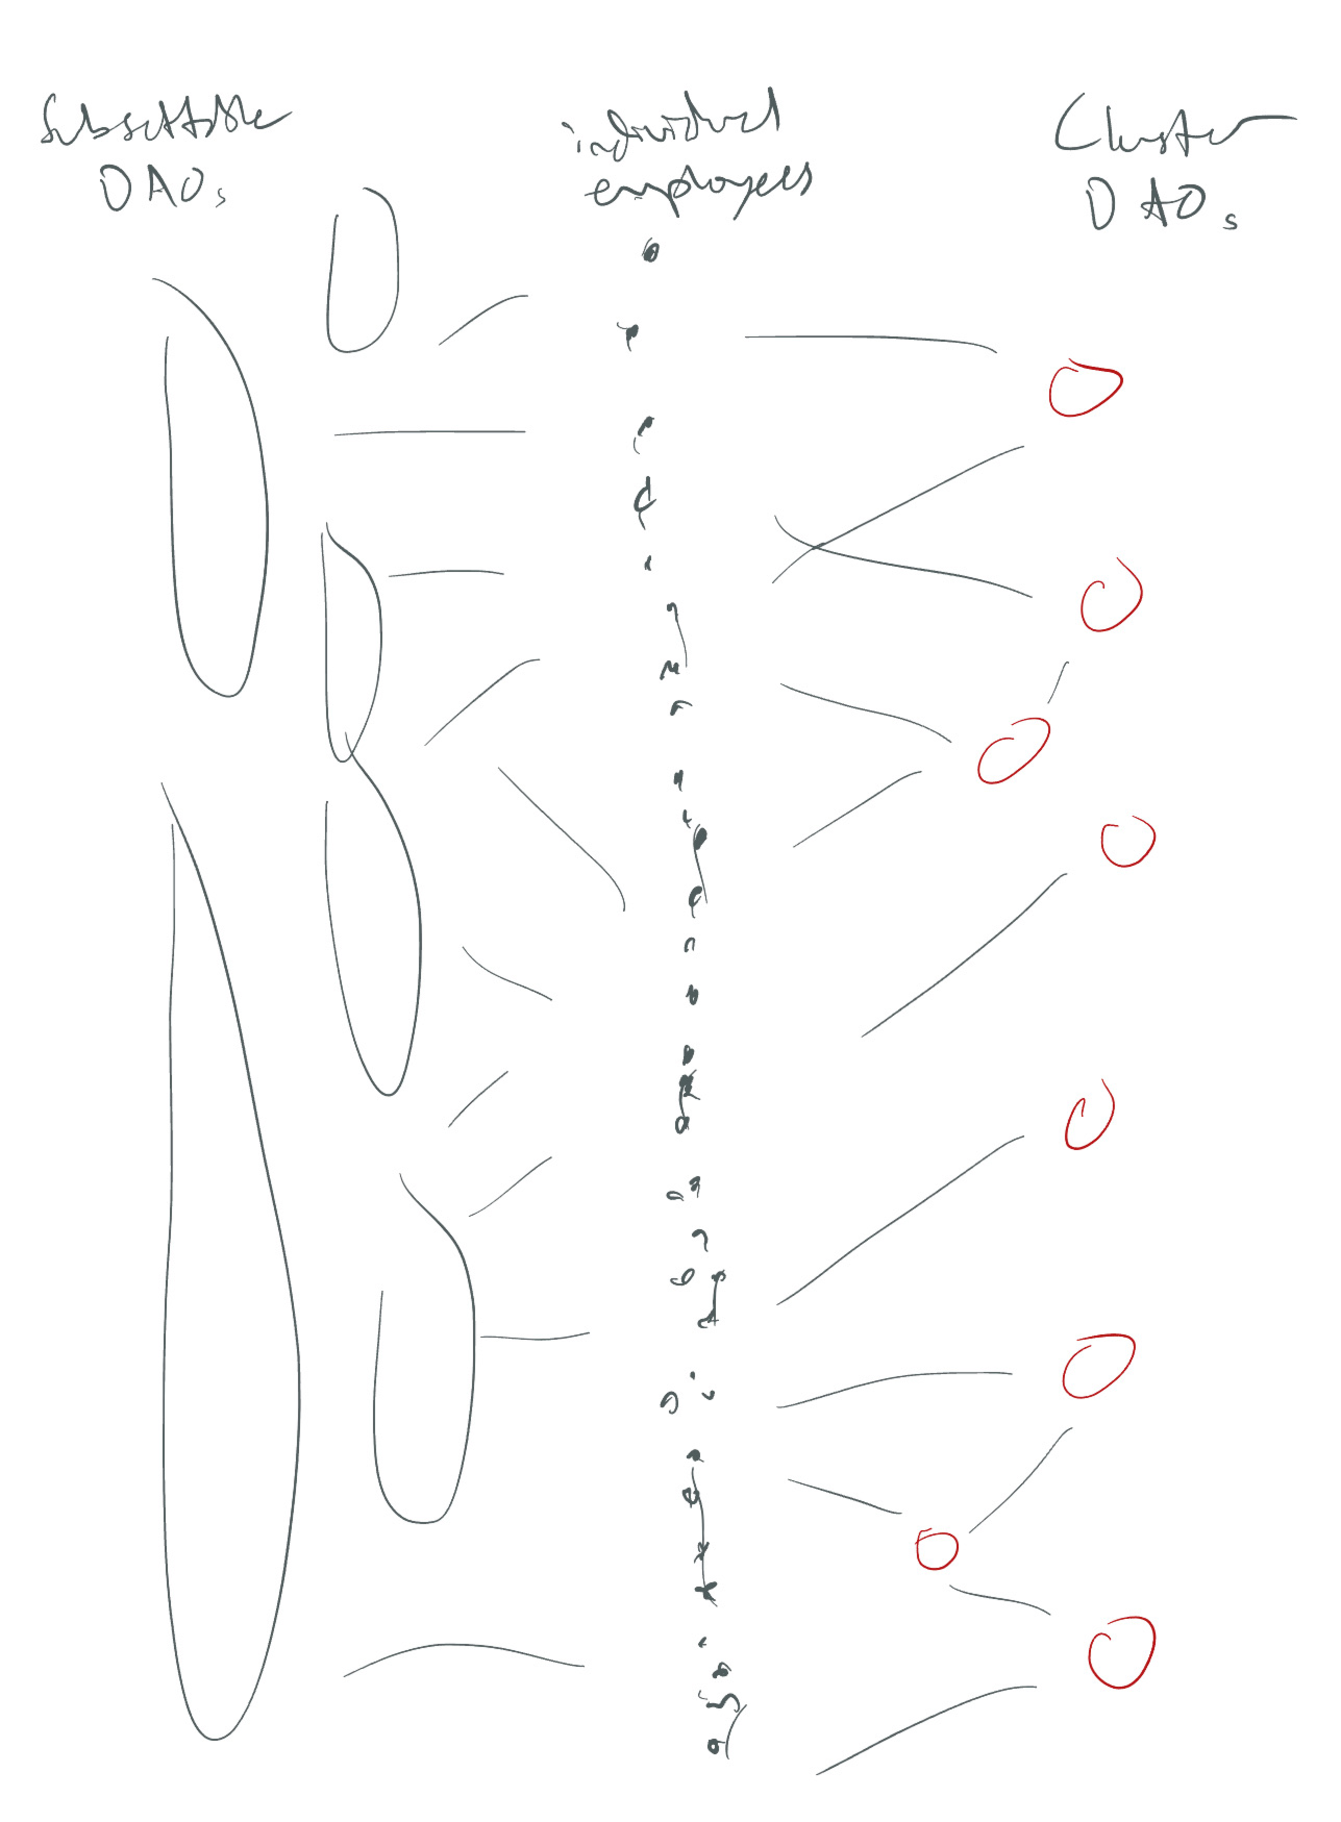
\includegraphics[width=\textwidth]{figures/IMG_1011.pdf}
    \caption{One potential enmeshment scenario. Clusters and subsets don't interact directly, but individuals use both to whatever extent suits them.}
    \label{fig:indirectEnmeshment}
\end{figure}

The other potential scenario is that of direct enmeshment between subsets and clusters, meaning a subset organization can become an RSN or an LN within a cluster.
An example of a subset acting as an RSN might involve a small family business or a worker's cooperative.
In the first case the family would define the subset as (the owner of the business / the business itself) and each of themselves as voting Members.\footnote{
    See Subsection \ref{subsection:customizability} for an explanation of how unequal ownership might function in the context of a subsettable organization.}
The latter case would function similarly, and the voting structure of subsets would be extremely useful to a worker's coop.
Similarly, a labor union is a great example of a subset that could function well as an LN within a cluster.
The individual laborers would vote on what RSNs to work for under what conditions, and how to distribute their income fairly.\footnote{
    A closed shop is a type of labor union in which employees of a company working in a position represented by the union are required to join the union. 
    An agency shop is a type of labor union in which employees of a company working in a position represented by the union are required to pay union dues even if they do not wish to officially join.
    It should be noted that there would be no way to prevent closed shop or agency shop arrangements with a given employer, as is done in some states.
    This is a result of SECCs being an instance of blockchain technology which is unregulated.\\
    \indent \indent \fullcite{closedShop}\textcolor{red}{*}\\
    \indent \indent \fullcite{agencyShop}\textcolor{red}{*}\\
    \indent \indent \textcolor{red}{citation for blockchain not being regulated}}
For depictions of both, see Figure \ref{fig:subsetCluster}.
This enmeshment of the subsets and the clusters concepts opens a whole new world for potential incentive structures, with the possibility of creating organizations that exist somewhere in between top-down companies and bottom-up cooperatives.

\begin{figure}[!ht]
    \centering
    \begin{tabular}{c|c}
    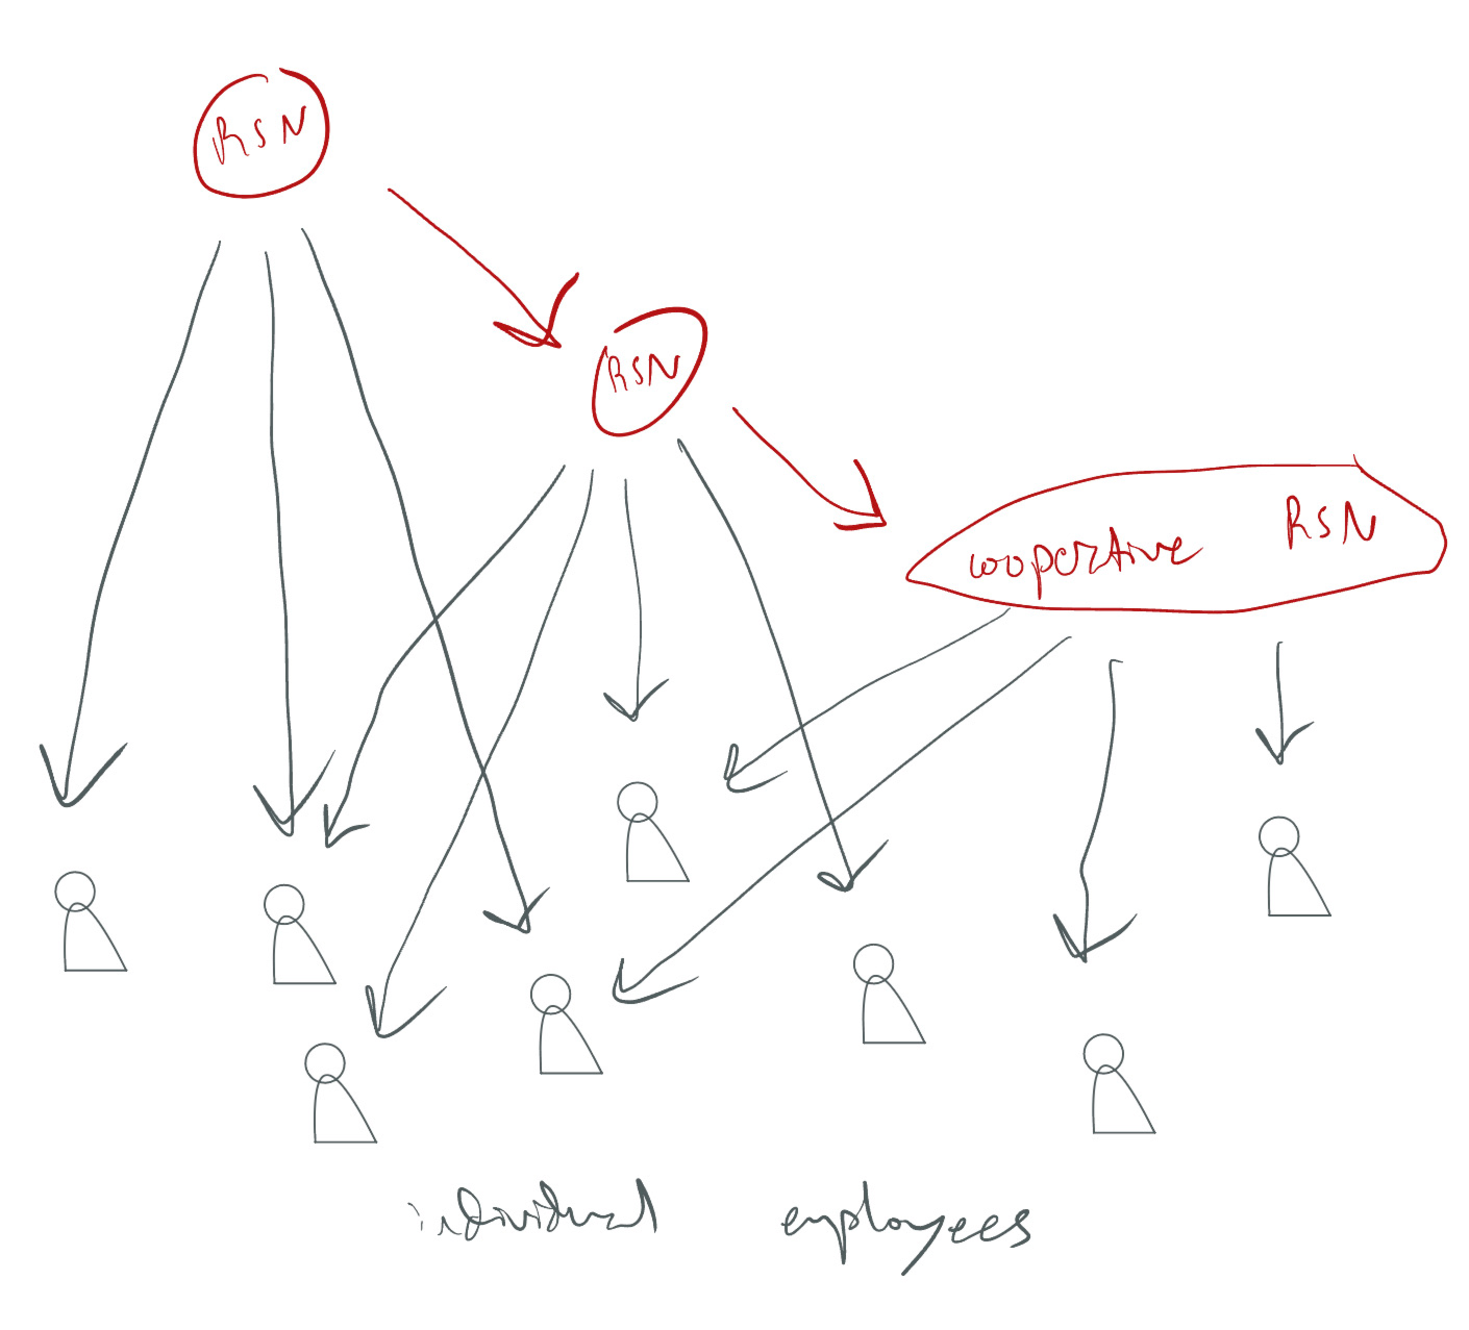
\includegraphics[width=0.5\textwidth]{figures/IMG_1013.pdf} &
    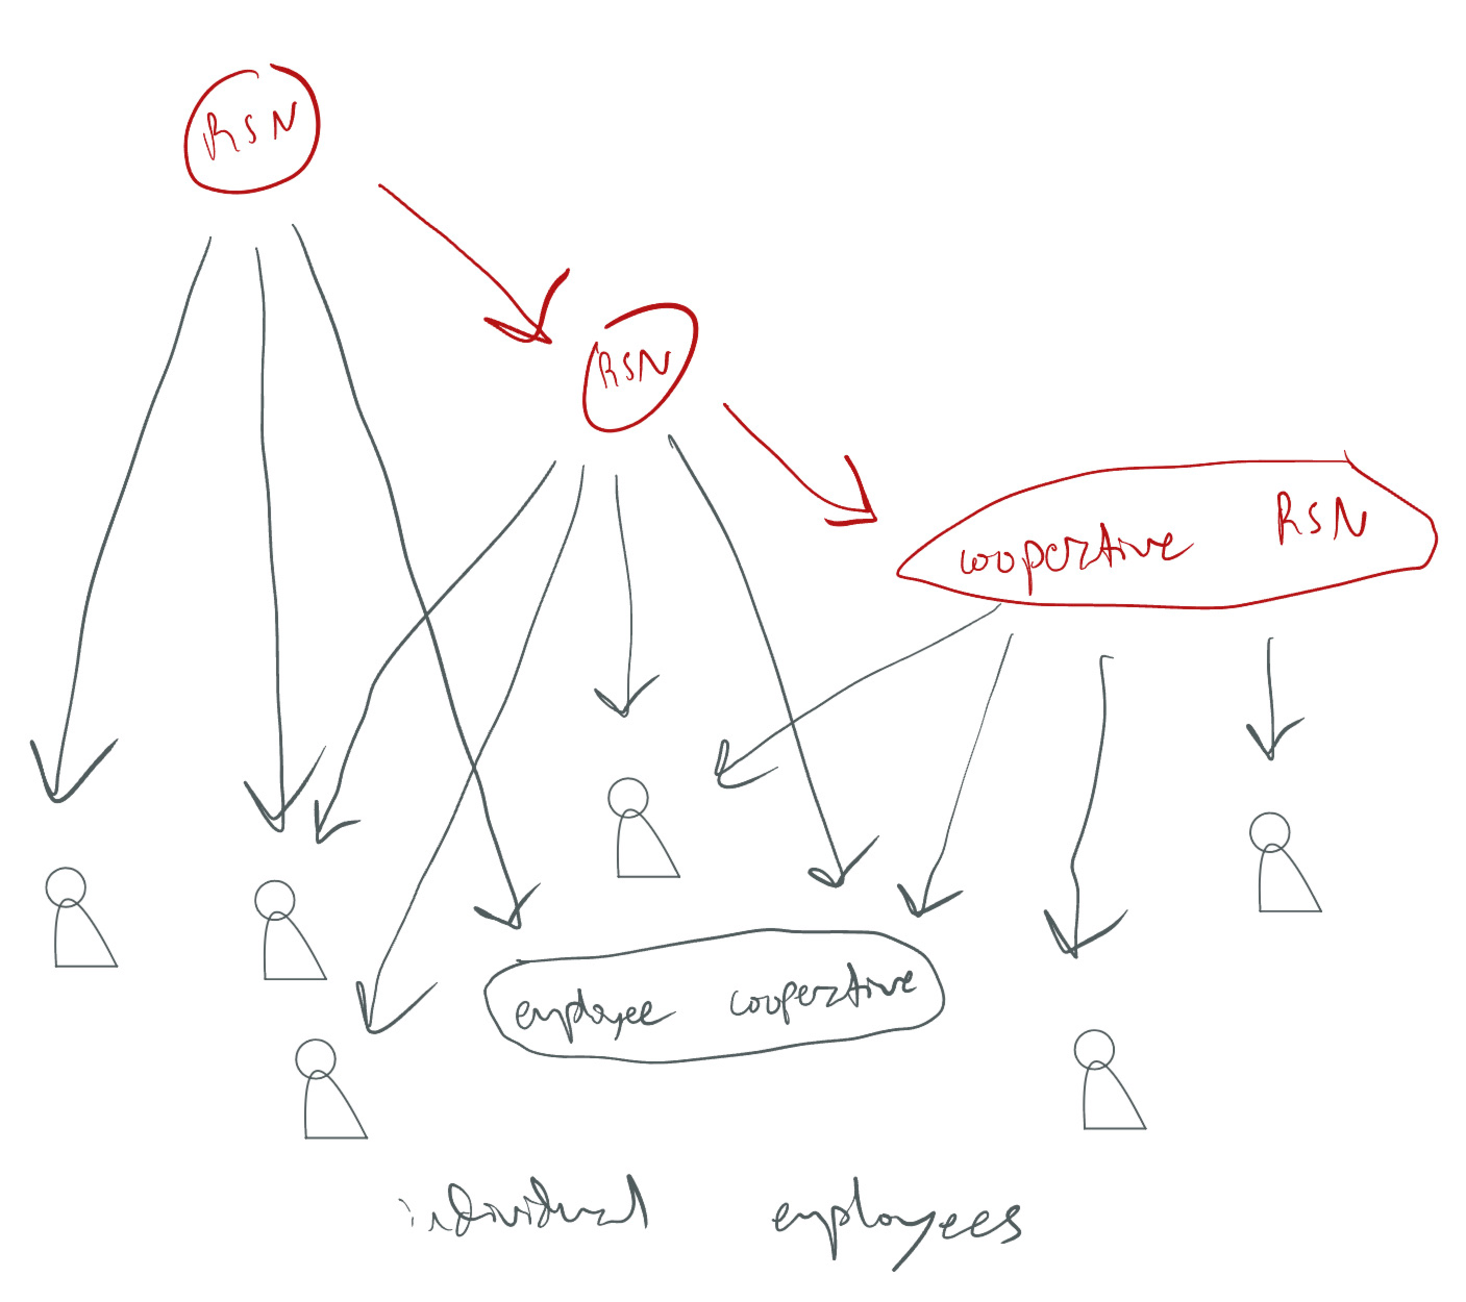
\includegraphics[width=0.5\textwidth]{figures/IMG_1014.pdf} \\
    \end{tabular}
    \caption{Caption}
    \label{fig:subsetCluster}
\end{figure}






\subsubsection{Enmeshing SECCs with Legal Contracts and Corporations}
\label{subsubsection:enmeshment2}

The real potential of SECCs comes in their various modes of interaction with legal contracts and corporations.
The world of the Crypto-Chad has avoided having anything to do with centralization and manual interaction; they prefer instead to create systems and incentive structures that exist entirely on-chain.
In order give blockchain technology uses beyond simple cryptocurrencies, a myriad of clever tricks have been conceived in order to enable some level of interaction with the off-chain world.
However, most are still restricted to entirely digital interactions and those that manage to draw some entanglement with the real world are rare and severely limited in the extent to which they do so.
See Subsections \ref{subsection:smartContracts} and \ref{subsection:DAOs} for examples of each, \textcolor{red}{respectively}.
Due to this insistence on decentralization, DAOs will by definition always be severely limited in their ability to interact with the off-chain world, an issue commonly referred to as the \_\_\_\_\_ problem.\footnote{
    \textcolor{red}{find a source for the problem where you have to choose between decentralization and blah blah blah, you can't have them all}}\par

SECCs on the other hand do allow for real-world integration specifically because they give up the decentralization dream.
Each RSN is a centralized source of revenue, usually incoming from the real world.
Each LN is either a centralized or decentralized source of labor, the performance of which could be verified by either decentralized on-chain or centralized off-chain means.
Subset Organizations are centralized when performing at a small scale, but as they get larger and subsume more subsets, the umbrella-organizations become closer to decentralized.
A given node in a cluster could be a DAO, but they need not necessarily be fully decentralized nor automated the way that a DAO is.\footnote{
    All squares are rectangles, but not all rectangles are squares.}
Now, what does this partial embrace of centralization mean for the potential enmeshment of SECCs with off-chain legal entities?\par

Let's look back at EvCorp, and the problem with the software developer becoming too powerful.
If I decide upon EvCorp's inception that this duty is too important to risk the programmer going rogue, then I could start a legal corporation to run in parallel with EvCorp, let's call it EvInc.
This company would do the actual hiring of the programmer, thereby retaining ownership and control of the website for myself.
They would essentially never be able to create their own RSN and break off from my goals.\par
\textcolor{red}{\begin{itemize}
    \item maybe instead of using the programmer as an example I can delve more into detail on the entrepreneur and the business that they make can involve some mission critical role
    \item need to emphasize that this should be used for cases when the business would not viably function without it.
    Enterprises of certain characteristics or of a certain size necessarily need top-down leadership, and we are allowing for the use of legal corporations/agreements so far as it can minimally perform this action
    \begin{itemize}
        \item At the end of the day, the goal is to do this as little as possible.
        The question is, can we design these things in such a way as to encourage that this is only done some optimal amount, or will everything just regress to a legal corporation because the profit hungry beasts will try to swallow up everything within reach?
        My intuition is that those which try to do so will be the equivalent of a ganandorf trying to fight shiek, so they'll be outcompeted.
        They won't be able to respond to changes in supply and demand as quickly and no one will want to work with them because SECCs just provide better wages and benefits
    \end{itemize}
\end{itemize}}

In many ways this example is just a regression back to a legal corporation, but it's important to emphasize here that this arrangement would not be ideal for all RSNs.
Rather, only those which are so interdependent as to not be able to function without complete control over one another would incorporate a legal structure, while some/most would maintain independence as RSNs.
It's important to note that the decision on which route to go is entirely up to the entrepreneur creating the cluster's first RSN.
When beginning a venture, they must ask themselves which functions need to be completely controlled versus which would work better with more flexibility and autonomy.\par

Along the same lines, when starting EvCorp's entrepreneurial ventures, it might be useful to incorporate legal agreements with the other RSNs.
Let's say I have a patentable idea and want to build a startup that develops a product based on it.
When I'm hiring an entrepreneur to implement my idea, it would make sense to have them sign a patent license.
When designing this license, I have two options depending on how involved in the business I'd like to be.
In the boring case, I give the entrepreneur complete business rights to manufacture, market, and sell this product in exchange for a percentage of their revenues.
I'd then use this royalty money to feed my own RSN, and allow the entrepreneur to conduct business however they like, whether that be as a traditional legal corporation or their own cluster.
In the more interesting case, I might instead give a factory owner a license to produce, but not to market or to sell to anyone except myself or someone of my designation.
I could then hire a marketer and design a contract licensing them to market the product, but not produce or sell it.
Finally, I would hire a sales/distribution team and license them accordingly.
These three separate entities would each consist of their own legal corporation which signs their respective license, but if they or I wish it then they could also open RSNs and distribute any relevant money through the EvCorp cluster rather than doing business with each other in a traditional manner.
I would further develop clauses in their contracts allowing me to rescind their license under pre-specified conditions designed to encourage them to function as RSNs.\par

A third and shorter example would be trademarks.
Let's say an SECC exists as a successful consumer-facing business, but they have no clear on-chain mechanism for developing a brand and preventing knock-offs from using their logo.
All they would need to do in order to have the same trademark protections as a traditional legal corporation is to have the owner of the central cluster file for a trademark and then license downstream nodes accordingly.\footnote{
    At first in order to enforce trademarks and copyright, clusters will have to utilize licensing contracts and/or legal companies as part of their structure.
    However, eventually we’ll be on a web3 system that can use software to prevent anyone from using an NFT they don't own on their website or digital product.
    For company logos specifically (a type of trademark), an SECC would make an NFT of their logo.
    \textcolor{red}{In order to make sure that no bad actors try to use an ever-so-slightly edited version (like an imperceptible color change) I’m sure there’s some kind of Fourier transform math that would allow us to detect and screen for ”similar” images.}
    Then on our web3 network we just decentralize the task of making sure that no one steals a logo.\\
    \textcolor{red}{sources explaining NFTs, web3, and fourier transforms as used on images.}}\par

A final example use for traditional legal structures has to do with avoiding legal liability.
Organizations that exists purely as SECCs would have each individual node responsible for their own mistakes.
A customer who has been wronged would have to sue the individual that they encountered in the transaction.
If instead the Members of the SECC were to open a legal corporation that was entirely employee owned, then when facing outward lawsuits they would equally distribute legal liability and have any damages be taken out of their collective profits.
In this way legal cooperatives could be used to avoid individual liability but still take advantage of the SECC structure in distributing resources and pay.\par
\textcolor{red}{\begin{itemize}
    \item might need to elaborate more on how a cooperative could have the secc structure determine how money moves within it instead of just sharing profits
\end{itemize}}

I hope it's becoming apparent how using legal arrangements can be a compliment to SECCs.
It should be noted that the current legal system is not meant for these uses, and as such there will be difficulties in implementation.
Furthermore, once governments do begin to notice SECCs, then we run the risk of poorly thought out regulations hampering their potential.
It is my hope that a hands-off approach will occur and work properly thanks to the complimentary nature of subsettable organizations and cluster organizations.
However, only time, trial, and error will tell.





\subsection{Customizability / Fluidity of Parameters}
\label{subsection:customizability}

The next big idea is not an altogether new concept, but rather an exploration of the inherent potential of SECCs resulting from their existence as smart contracts.
As discussed in Subsection \ref{subsection:smartContracts}, smart contracts are turing complete, meaning they are full fledged computer programs capable of executing behavior of any necessary level of complication.
They do exist entirely on the blockchain, so they can only influence and act within the blockchain, but this still leaves a wide variety of potential.
They are essentially similar to legal contracts in that any two parties can write one and enter it upon reaching an agreement as to what its terms should be.
However unlike their government enforced alternative, smart contracts execute their clauses automatically and in such a manner that is uncheatable by the parties involved.
This means that rather than having to enforce terms after they have been broken, the terms of a smart contract cannot be broken in the first place so long as the necessary implementation actions can be performed entirely on-chain.
It is this infinite customizability paired with the ironclad nature of the execution that makes smart contracts so powerful.\par

In this section we describe all of the dimensions along which SECCs can vary from one to another.
You will hopefully find it quite striking just how different from each other they can be.
This inbuilt variation means that rather than being one specific new thing for society to implement, the idea of SECCs is to have an unending landscape of different ideas, structures, and implementations to compete with one another.
It is this survival-of-the-fittest aspect that will allow SECCs to adapt dynamically to specific goals and market conditions.
Rather than proposing one ideal for all others to follow, the ideas in this paper instead wish to create a structural playground for entrepreneurs, tinkerers, and dreamers to best pursure their ideals within.
The following are all important dimensions along which SECCs can vary:\par 

\begin{itemize}
    \item \textbf{Purpose:} 
    Traditional legal bodies make distinctions between for-profit firms, cooperatives, community organizations, charities, etc. Individual nodes within an SECC can be any of these or even more than one at the same time.

    \item \textbf{Implementation Incentive Structures:} 
    Nodes within SECCs can use any combination and degree of direct versus indirect funding,\footnote{
        An example of indirect funding in EvCorp would be me paying the PhD to make video lectures for the programmer's website.
        If I were to give money directly to the programmer they might not use it according to how I wish, whereas If instead they receive videos then they might as well post them.} 
    centralized versus distributed capital ownership,\footnote{
        Decentralized capital ownership refers to each node owning the capital they have direct access to, such as the programmer with the website.
        An example entailing centralized capital ownership is the scenario where I establish the legal corporation EvInc to hire the programmer and therefore keep the website that they produce within my full control.
        Traditional legal corporations practice centralized capital ownership.}
    and legal enforcement to incentivize other nodes to behave in a certain way.
    In contrast, corporations use primarily direct funding and legal enforcement for encouraging all desired behavior plus centralized capital ownership for intragroup incentive structures.

    \item \textbf{Voting Structures:} 
    Subset organizations can potentially have wildly different systems for decision making far beyond what has been discussed in this paper.
    The modular \_\_\_\_\_ system detailed in Subsection \ref{subsection:BestFriendsUnion} is my personal favorite for complicated networks of sub and umbrella-groups.
    In contrast, legal corporations usually either have an owner that makes all decisions or stockholders far removed from the particulars of the business vote with their only incentive being profit.
    \textcolor{red}{\begin{itemize}
        \item need to go back and strictly name/define the modular \_\_\_\_\_ voting system.
    \end{itemize}}

    \item \textbf{Ease of Separability and Combination:} 
    To the extent that individuals, cluster nodes, and subset groups are enmeshed with each other, there can be rules defining exit and entry conditions.
    For example, BFU might require a deposit upon entry that would not be recovered if an individual were to leave suddenly and without giving proper warning.
    These incentive structures will be designed to make SECCs either more static or more dynamic, depending on whether their purpose benefits more from consistency of application or from adaptability to changing conditions.
    Corporations in contrast have to go through legal hoops in order to split or merge, and are therefore stuck being relatively static.\footnote{
        Difficulty in the latter makes sense insofar as it prevents the formation of monopolies, but such restriction becomes unnecessary once you introduce distributed capital ownership and easy separability.
        \textcolor{red}{consider finding biology words for separability and combination like mitosis or something.}}

    \item \textbf{Profit Distribution:}
    The list of ways a cluster organization could choose to distribute excess profit includes all the methods pursuable by legal corporations such as to a single owner or to investors, plus that of distributing to the newly defined capital owners (RSNs) or that of equal profit sharing as is done in cooperatives.

    \item \textbf{Direction of Decision Making:}
    Legal corporations utilize top-down decision making, whereas DAOs are bottom-up.
    SECCs can implement either but more commonly exist somewhere in-between with RSNs calling the shots.
    Thanks to their modular structure, SECCs can build themselves out of a frankenstein of subcomponents that might each implement different decision making strategies.
    This can be thought of as the extent of use of and/or enmeshment between subsets, clusters, and legal entities/agreements.
\end{itemize}

\noindent For a depiction of the six aformentioned dimensions upon which SECCs can differ from one another and how their range of potential compares to DAOs and legal corporations, see Figure \ref{fig:variation}.\par

\begin{figure}[!ht]
    \centering
    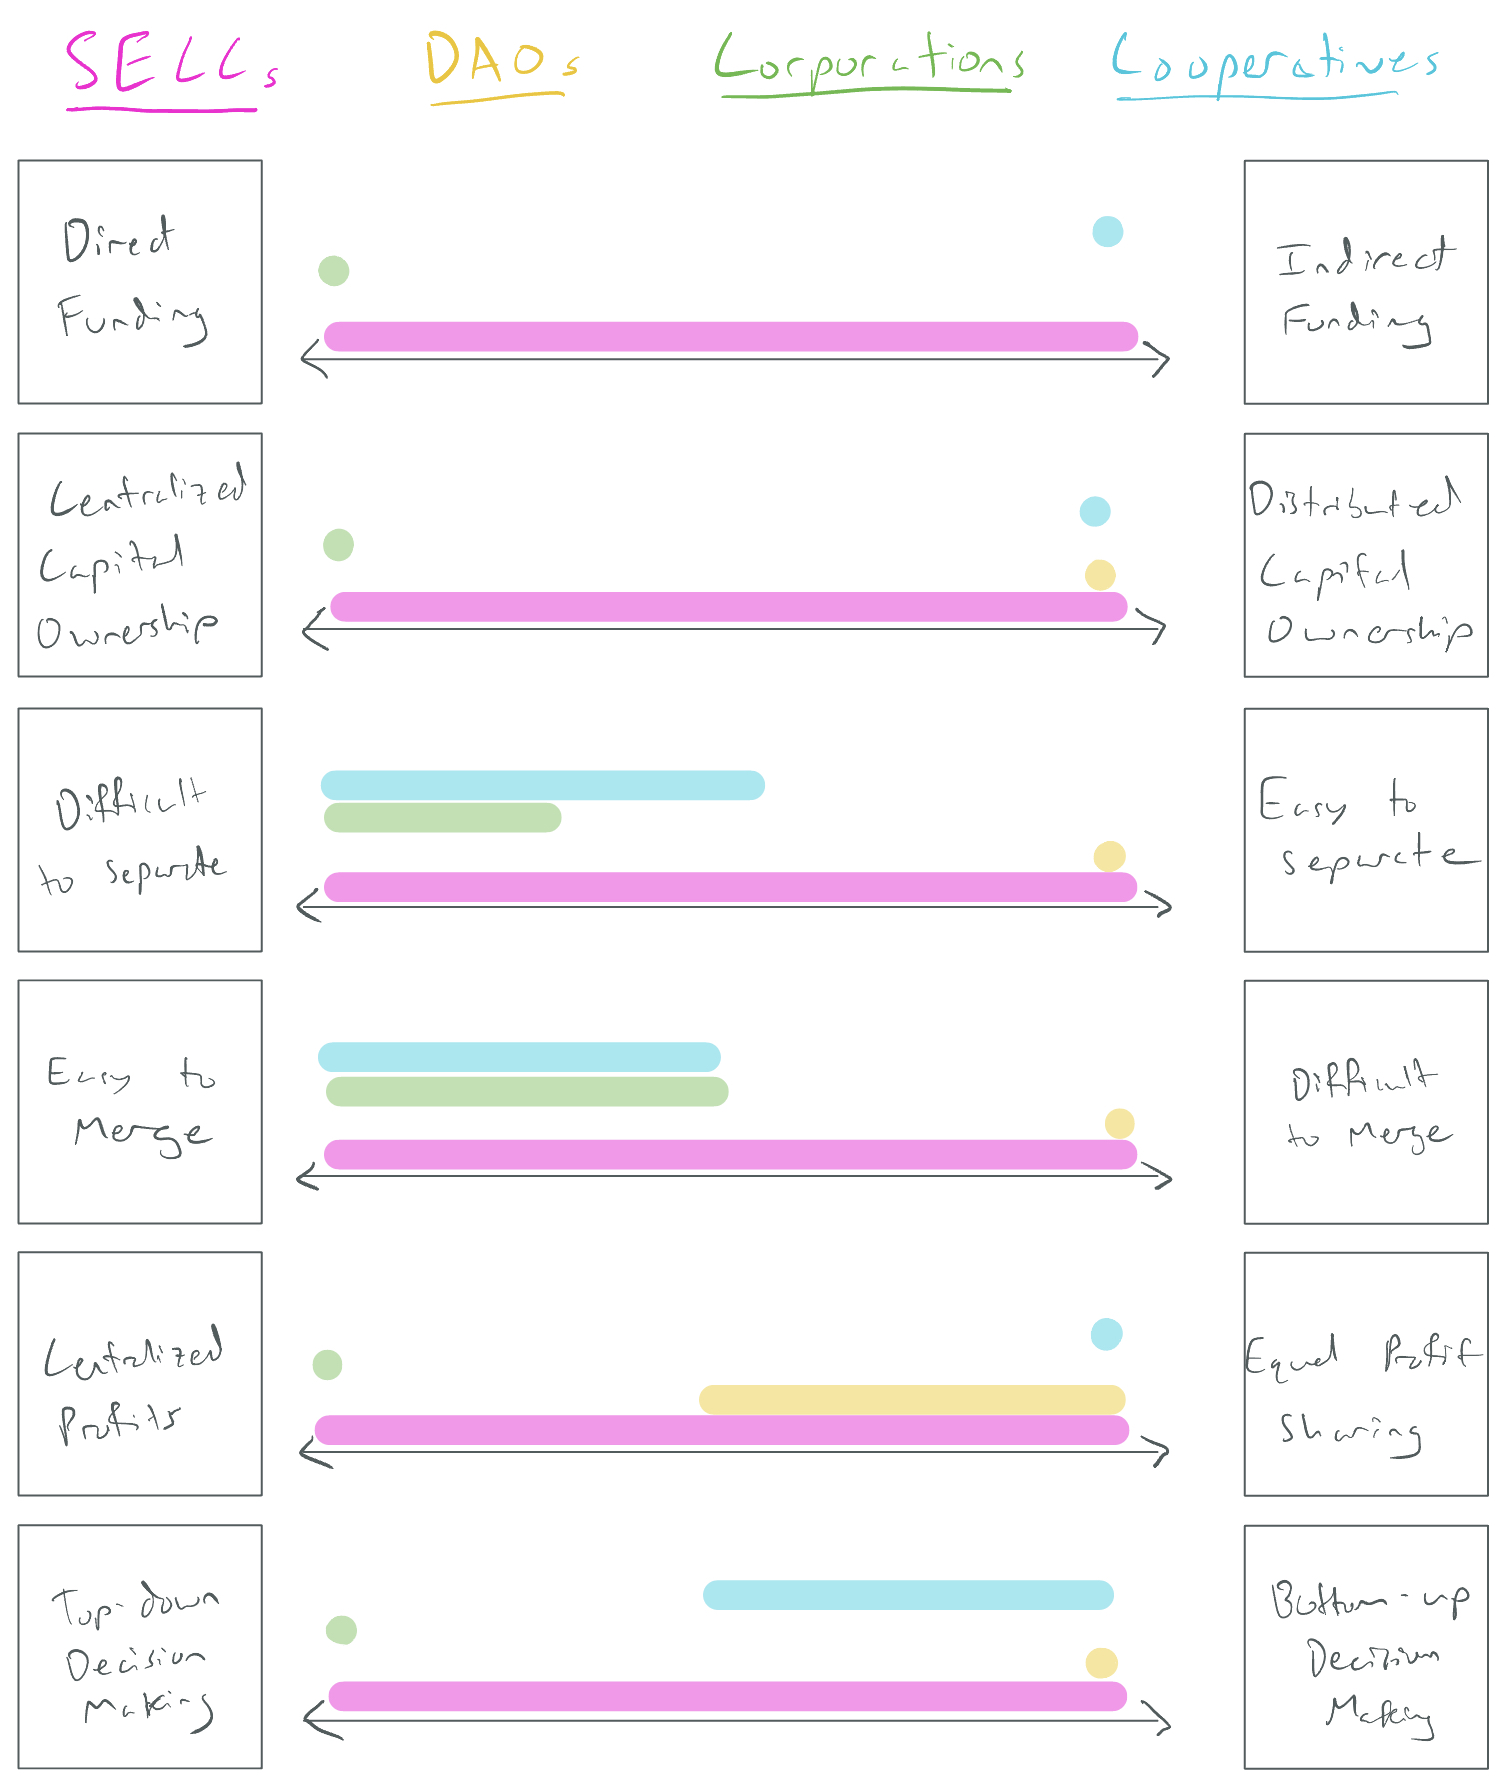
\includegraphics[width = 0.8\textwidth]{figures/IMG_BB0DCC4686FC-1.jpeg}
    \caption{This plot doesn't have any corresponding numbers it's just my initial sense of where each organization type lies.}
    \label{fig:variation}
\end{figure}

The specific makeup and settings of a given SECC are determined at the level of the individual nodes making agreements with one another.
They make such choices based on their goals and what settings they think will best help them achieve such pursuits. 
In the beginning there will be a confusing, chaotic playground of ideas and implementation methods competing with each other, but eventually patterns will emerge of best-practices for each potential organization's purpose.
For example, as sizes scale there may be more of a need for top-down decision making in profit-seeking firms, whereas bottom-up processes may work better for ventures involving collective action as they grow in size.
These naturally emergent, goal-specific best-practices can be standardized into templates to make entry easier for new users.
For a group of close pals that are late to the SECC party, they can just use the template created by Best Friends Union rather than debate the specifics of every single setting available to them.
In this way an extremely complicated system can be made simple for the masses who can rely upon the wisdom earned in trial and error by the tinkerers that were early to the party.\footnote{
    "Civilization advances by extending the number of important operations which we can perform without thinking about them."
    \fullcite{hayek1945use}}

These concepts of variability, tinkering, trial and error, use of templates, and competition allow us to make an analogy to evolution.
Universal Darwinism is a theory stating that the evolutionary dynamic first described by Darwin can actually apply to non-biological systems if they meet certain prerequisites.\autocites{UniDarwinism1, UniDarwinism2}
While no two businesses to date have ever been identical, and comparisons between Adam Smith's invisible hand and Darwin's survival-of-the-fittest paradigm have long been made, it is important to stress that there are more dimensions along which SECCs can vary from each other than traditional businesses can.\footnote{
    \textcolor{red}{sources for wealth of nations, something comparing hand to evolution}}
These new playgrounds for variation are designed to enhance and speed up the "evolutionary" process, hopefully thereby giving us firms that can actually out-compete their predecessors.
If SECCs do in fact have a competitive advantage, then their use should naturally emerge without the need of any government or otherwise organized assistance.\par

To further the evolution metaphor and continue along the theme of the importance of variation, we can look at biodiversity (firmdiversity) and the health of the ecosystem (economy).
In ecology (economics), healthy ecosystems have a plethora of different species (firms) competing with one-another; fewer species necessarily leads to higher reliance of the ecosystem on each species, meaning all of the eggs are in one basket.
Analagously, economies do poorly when reliant upon a small number of industries or even firms.
For example, see the negative consequences of when nations become highly dependent on oil exports or that of a similar natural resource.\footnote{
    \textcolor{red}{sources about the resource curse}}
Another would be the 2008 financial crisis and following occupy wallstreet movement in which the largest American banks were deemed "too big to fail."\footnote{
    \textcolor{red}{sources}}
That very phrase blatantly admits over-reliance on too-few firms.
Economies are better off when they put their eggs in multiple baskets rather than in a small number of industries, banks, etc.
These single/few points of failure are dangerous because every institution will eventually fail at some point.
SECCs on the other hand can help avoid this issue.
This is because individual nodes within a cluster have the potential to survive the downfall of a related node; this is in contrast to legal corporations where the failure of one critical component will take the ship down with it.


\textcolor{red}{\begin{itemize}
    \item solves Taleb’s biodiversity point. This system of “organic”, evolving companies would allow for a few big players and a huge biodiversity of tiny companies
\end{itemize}}





\vspace{1in}
\begin{center}
\color{red}
\textbf{\textit{End of somewhat finished portion.}}\\
\textbf{\textit{Everything from here on out is basically brainstorming.}}\\
\textbf{\textit{Much of it was written months ago and has not been looked at even a second time}}
\end{center}

\subsection{Feasibility / Conditions for Success}
\label{subection:Feasibility}

\textcolor{red}{\begin{itemize}
    \item WE NEED THE UNIQUE NAME IDENTIFIER TOKEN THINGIES FOR EACH PERSON
    \item some kind of reputation system
\end{itemize}}

\textcolor{red}{for whatever cryptocurrency this is based on, all the users need to full on commit to only using it as much as they’re able to. 
It’s important to separate from the regular currencies as much as possible in order to not get pulled into their drama}
\textcolor{red}{\begin{itemize}
    \item separation takes us off their business cycle
    \item separation partially isolates us from their black swan events, and hopefully we're inherently less susceptible to black swans
\end{itemize}}






\subsection{Abandoned Subsection Ideas}

\textcolor{red}{No longer gonna give these their own subsections but some of the thoughts might still be useful}\\

\noindent \textcolor{red}{Cooperative DAOs (voting)}
\label{subsection:cooperative2}
\textcolor{red}{\begin{itemize}
    \item not a new idea in the DAO space
    \item volunteer participation / no single ownership structure lends its way to equitable groups, but technically some groups could have a top down command structure
    \item whereas earlier I broadly described cooperatives, here I'll detail the implications that a cooperative structure has for SECC's, essentially the interaction effects of S*Coop and Cluster*Coop
    \begin{itemize}
        \item intergroup cooperation
        \item \& the more obvious intragroup cooperation
        \item it is my belief that these interaction effects are so powerful as to discourage dictatorial groups
        \begin{itemize}
            \item does this apply all the time, or only most of the time?
            \item a "SEC DAO" (missing the Cooperative C) firm would be easily out-competed in the labor market and have trouble hiring quality candidates.
            \item Less obvious but more notably, said firm should also eventually run into difficulties in the consumer market as such a decision would massively hinder the firm's flexibility, essentially handicapping it in comparison to it's full fledged SE\textbf{\underline{C}}C DAO competitors.
        \end{itemize}
    \end{itemize}
\end{itemize}}

\noindent \textcolor{red}{less decentralization / more real life (necessary component)}

\textcolor{red}{\begin{itemize}
    \item current DAOs are just smart contracts existing on the blockchain, with incentives set up so that randos will help out. 
    I want to incorporate that with real-life working relationships so that rather than start companies, entreprenuers will want to start SECCs because it gives them more fluidity in company structure
    \item including the legal system??? 
    do we still start companies and everyone is a contractor or something, which is no longer an issue because they can get their health insurance from an SECC? 
    idk dude
    \item but in certain ways, separation from the rest of the economy is absolutely necessary. 
    the more of the economy that converts to SECC's, the greater advantage they will have because they'll have greater potential to mix \& match and evolve. 
    So how do current legal \& tax structures intertwine with this?
    \item should this subsection just be a piece of the customizability section? 
    or maybe in the prerequisites section?
    \item stress importance of people fully committing their economic lives to it. 
    Might be a way to get the world to actually convert to cryptocurrencies as a currency rather than as an investment tool. 
    Same way some ppl insist on only buying american, the users need to insist on only doing business with SECCs whenever possible
\end{itemize}}












\section{Addressing the Flaws of Centrally Planned Economic Systems}
\label{section:CentralFlaws}
\subsection{Information} 
Hayek detailed how communism just can't match the information efficiency advantages of a free-market system with prices. \autocite{hayek1945use}. 
To summarize his argument, there's no way that socialist central planners can know enough to efficiently predict how much of what good should be created and where it should be distributed to. 
Each worker on the assembly line has tiny bits of useful information about how much their factory can produce at what quality by what time and at what opportunity cost, and each consumer has unique needs also not knowable by a central planner.
Any attempt at guessing the aggregate values without all of this disorganized, distributed information is doomed to failure resulting in the classic "waiting in lines for bread" story of communism. 
This problem is solved because we're still using capitalism's price information communication structure. \par
However, this will be a limit of our system compared to previous forms of socialism.
Because people join groups willingly, chances are they will group together with people of similar income brackets and therefore more expensive goods will still usually be out of reach to the same people they've always been out of reach for. 
The magnitude of the effect this system has on wealth inequality will depend on the culture; how willing will people be to group up with someone who makes significantly less than them?

\subsection{Innovation} 
Socialist systems lack incentive for entrepreneurs to innovate.
Here, that incentive may be diminished since any increased earning will be distributed somewhat equally among your group.
However, I believe that if you're grouping together with people who you know and trust and care about to a certain extent then you'll likely still feel incentivized to earn money. 

\subsection{The Welfare State}
This system essentially circumvents some of the issues of welfare states. 

\subsection{Succumbing to Sloth}
should this section just be combined with the welfare state section?\\
lazy people won’t do well here because in order to be in a group you have to convince the rest of the group that you’re worthy. 
Convincing the government involves a lot of wasted time, energy, and money in the form of proving that you’re applying for jobs and having a bureaucrat confirm that you actually are. 
A given group might allow some people to be unemployed if they’re really kind and the unemployed have a good reason, but odds are that freeloaders will not have an easy time taking advantage of this system. 
Any group that designed itself in such a way as to encourage free loaders would inevitably collapse on itself as all the people who actually pulled their own weight left

\subsection{Bureaucracy}
there’s no wasted bureaucracy money because everything is automatic. 
I mean some effort is put into designing the contracts and enforcement in the form of group voting but I imagine that’s minuscule compared to the drain that bureaucrats have on the economy. 
Maybe include some stats and sources if I want to make this an actual sub subsection instead of a sentence or two

\subsection{Revolution}
This is only included in this section because marx talked about it. Really it applies to any significant change to the status quo. \\
Why would one risk their life for a benefit that will be evenly distributed among all? 
That's why all revolutions have been led by people on the cusp of power and resulted in them gaining more power. 
This method is sick because it doesn't require revolution, it can spontaneously emerge and exist within/alongside any society

\subsection{Corruption} 
need an analogous subsection under capitalism section \\
This issue is essentially not applicable here. 
Terms of the contract are agreed upon ahead of time before willingly joining a group, and the blockchain technology ensures that it's impossible to straight up steal funds or anything.
If we could pay our bills directly in crypto, then we'd even be able to ensure that people spend their money on what they're supposed to.
However that might not happen for awhile in which case members would have to receive a monthly or biweekly 'allowance' and be trusted to not spend it all on crack. 
There will be some scammers creating groups in the beginning but even that should be few and far between as long as people read their contracts and only choose to group together with people they know and trust. 

\begin{figure}
    \centering
\begin{tabular}{cc}
   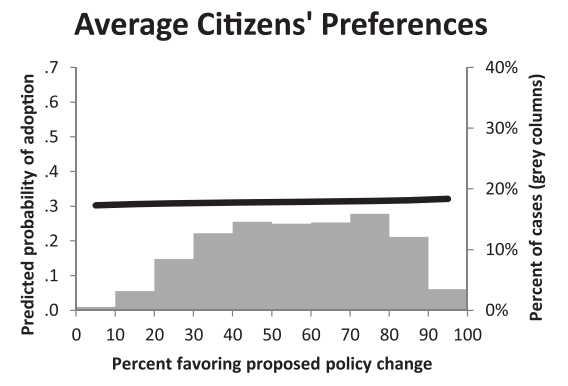
\includegraphics[width=0.5\textwidth]{figures/Capture.PNG}  & 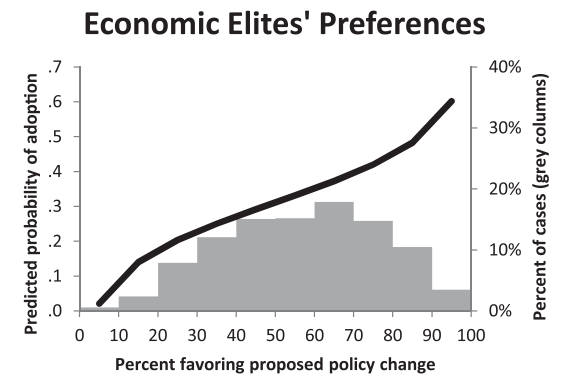
\includegraphics[width=0.5\textwidth]{figures/Capture2.PNG} \\
\end{tabular}
    \caption{Caption\autocite{gilens2014testing}}
    \label{fig:my_label}
\end{figure}


\section{Addressing the Flaws of Free Market Systems}
\label{section:FreeFlaws}
\subsection{Wealth Inequality}
Wealth inequality is probably the biggest problem with our modern day iteration of capitalism. 
This cryptocommunism idea does not make everything equal, but hopefully goes a way towards evening things out. 
I think the early adopters of actual communists will in theory have no issue joining groups with people who earn significantly lower than themselves. 
However it's that first wave of regular people that would find the idea of taking a willing pay cut difficult, so for as long as we all still have a greedy capitalist mindset this system is going to have to provide some benefit to even the richest person of a group in order to encourage them to join and start making an impact on wealth inequality. 
Not sure how to do that. 
Cultural pressure? 
Cheaper than buying regular insurance even for a rich person? 
Will rich people make their own groups exclusively for the rich for some reason?


\subsection{Market Failure} 
This section is not directly addressed so we still expect gov’t to regulate cases of market failure. 
HOWEVER, we know that actual people rather than capitalists are willing to the the right thing. 
So it’s not a guarantee but there’s a chance that employee ownership of companies would SOMETIMES fix these problems

\subsection{Negative Externalities} 
Environmental damage might end up being the downfall of capitalism (and the earth I guess lmao). 
This issue is not addressed by cryptocommunism as the markets are left untouched. 
That being said, I have a suspicion that it might trigger change toward a more collectivist mindset which would then exert pressure on firms to behave differently. 

\subsection{Boom and Bust Economic Cycles} 
The tendency for markets to crash is a big hamper on society and I think the movie The Big Short even quoted some statistic saying that creashed result in tens of thousands of people dying or something. 
This issue is not directly addressed by cryptocommunism since markets are left untouched. 
However, I think stabilization of everyone's income would make the busts more manageable on an individual level. 
Rather than losing your job and being entirely SOL, you losing your job instead results in a moderate income decrease for everyone in your group.
Classical economic theory actually states that recessions wouldn't really matter and would just be an effective change in price level if only people were willing to let their wages drop a bit rather than sacrifice the employment of some of their coworkers. 
As a sidenote, I imagine other members of the group would feel they have incentive to help a group member who lost their job find another one, so a large enough group may provide serious employment stability advantages.

\subsubsection{Busts}
when ppl lose their jobs the group wage just dips a bit. Classical econ theory says we would be able to avoid recessions if ppl would take a dip in wages instead of letting a certain percent of workers go. 
So this system would effectively mitigate recessions in a way that classical theory would love
\subsubsection{Booms}
when the boom starts, usually everyone is earning more and spending more BUT the poorest ppl are the actual driver of the economy since they spend a larger percent of their income. 
If people hop on to the wealth distribution idea then this idea should 

\subsection{Unhampered Growth}

\subsection{Materialism and Mental Health}






\section{Brainstorm of specific details / potential instantiations}
\label{section:Brainstorm}
\begin{itemize}
    \item all people should start off in small groups rather than directly joining a huge one (maybe idk). 
    The ledger of small groups should be publicly available or at least available to whatever larger group the tiny group wants to join. 
    I say publicly available because if an individual wanted to join your group and we’re not doing sub/super groups then it’d be nice to check the ledger of some tiny group they were in before. 
    This system really needs to be built off trust so starting with tiny groups only among people you know just makes too much sense. 
    Maybe I should have a section discussing my thoughts on the recommended ways to enter/start the game. 
    Really like small groups with friends \& family / known coworkers, and then medium groups with lots of shared acquaintances.
    
    \item Ok so to incentivize people to participate well in groups, obvi you need incentives built into the initial contract. 
    But on top of that, maybe a reputation system. 
    it’d be an overall reputation score for every Member as well as a breakdown of what types of groups they’ve shown to be trustworthy in.
    
    \item The parameters that a group chooses might limit what subgroups or supergroups it can link to.
    
    \item When you join you commit to future payments and a sizeable security deposit or something. 
    I'd imagine if you don't submit your payment for the month then the blockchain program just doesn't give you the monthly payout/benefit, or doesn't give it to you for that month and the next.
    Idk, people can customize and figure out what incentives work
    
    \item Each Member effectively needs its own crypto wallet that is only accessible by the smart contract running the group. Obviously a group vote can override and take money out
    
    \item for BFU allowances will likely be a bulk regular amount with loose recommendations on how to spend it (x\% to rent, y\% to food, etc.).
    Eventually when the entire economy is using crypto then the smart contract that runs BFU could actually force u to spend your money in certain ways which would be amazing for people with poor self control
    
    \item Of course people are still going to group together with others who are in the same tax bracket. 
    Maybe the subgroups can distribute wealth evenly while big supergroups incorporate a progressive tax structure that helps a tiny bit with inequality. 
    
    \item Groups vote on things and specify rules for legitimate voting. 
    What percent of members need to participate in a vote in order for it to be legitimate? 
    Are there time limits on when you have to get a vote in by? Do those time limits vary based on the topic? 
    What percent of people need to vote yes for a new idea to go through?
    
    \item Supergroups that exist for reasons other than wealth distribution might find a flat rate tax structure useful.
    For example, maybe in a health insurance SECC every subset just contributes 10\% of their income then has health costs fully paid on a need-blind basis. 
    Obviously rich people would end up paying more, but this might not be such a big deal in exchange for the huge amount of money and diversification that poor people in aggregate can provide.
    Obviously a progressive payment structure would be hard to get people to willingly commit to, but I imagine some very nice rich people might be willing to do a flat percentage rate.
    
    \item You might want to choose your group based on proximity or some other variable that changes with time (maybe you're always in a subgroup with your roommates at the time).
    Participation should always be voluntary, and anyone can leave a group at any time they want. 
    However, in order to discourage leaving without proper warning and preparation, there should be predetermined financial punishments for leaving early that are agreed upon when you first join the group.
    For example, maybe a 2-month warning becomes regular and if you give less warning than that then you lose your security deposit or something
    
    \item Caution: this structure has zero say as to how off-chain companies function if you're still employed by one of them. 
    In theory they are unchanged and still pay you regular wages, you just decide what to do with those wages and they may be incentivized to stop providing healthcare or other benefits that you get through your group. 
    I strongly recommend against letting your company form a group and joining it. 
    They generally do not have your best interests at heart.
    I know it seems like they do because they already give you health insurance and whatnot, but they only do that because they have to.
    The blockchain is unregulated and they will take advantage of that fact.
    However, theoretically if you agree with the terms of the contract proposed then there's no real reason to say no since your employer who just happens to be creating a group for their employees has no ways to break that contract.
    
    \item This stuff might be picked up quicker among people who are self-employed as an alternative to buying health insurance and whatnot on their own. 
    People who already have health insurance through their employer would obviously be less motivated to join since they'd be essentially foregoing that value that their employer provides.
    
    \item At the initial creation of a group you should be able to set a minimum group size. 
    If not enough people sign up initially then the group just never gets made because you wouldn't want a group with too few people, that might not be effective.
    Along with that, maybe there should be some kind of pre-planned shutdown sequence in the case that too many people leave for the group to still be able to function properly. 
    
    \item There should be a system for smoothly transitioning someone to a new group when planned out ahead of time to avoid temporarily being without group safety and to minimize blockchain resources taken up. 
    
    \item At the heart of this effort is providing as much customization as possible. 
    We don't know what parameters will result in these projects succeeding, and it is highly likely that those parameters will vary person to person and group to group
    
    \item The voluntary and modular nature means that inequality from capitalism will never fully go away, just hopefully get subdued a bit. 
    This is of course good to a certain extent because the price system is what allows us to efficiently allocate resources and incentivize innovation, and without a bit of inequality the free market would lose much of its ability to innovate and realocate resources efficiently. 
    There is also the possibility that I'm not fully comprehending the system and it actually makes things worse.
    I think that scenario is only likely to occur if the government steps in and tries to limit a single aspect of this.
    
    \item If everybody’s paycheck came in at the same time, like Friday evening every other week for example, then wouldn’t there be a way to set up a direct deposit to a bank account, then automatically spend your entire paycheck on etherium, immediately have that go to the group and get redistributed, and then immediately sell your eth and put your post-redistribution paycheck back into your bank account? 
    I don’t think all bank deposits would go through at exactly the same time but that’d trim any issue of etherium’s variability down to a few hours. 
    Or if everyone waited until all direct deposits were in their account they could press a “ready” button on whatever app. 
    Then once everyone has hit ready it could all happen within a matter of seconds.
    This would be useful during the transition period where most of the economy still exists off-chain and people are just trying to get some benefit from the automation capabilities of this technology.
    
    \item "Civilization advances by extending the number of important operations which we can perform without thinking about them."
    - Friedrich Hayek \autocite{hayek1945use}\\
    idk how i'm gonna make this thing simple.
    fuck
    
    \item “In their view, and following Hayek, the hedonism that corrodes the foundations of society finds its origin in debt and easy credit. 
    A deflationary currency discourages consumption, since the value of the money you have grows with every passing day that you don’t spend it, and a currency that prohibits the creation of money from fractional reserves discourages credit, since the only way to borrow money is to take it from existing reserves that have been hard-earned by saving. 
    Bitcoin is thus intended to encourage the virtues of endurance, continence and frugality that characterize strong men and solid societies, unlike all those ‘soft currencies’ associated with periods of moral decadence, military clashes and economic decline.”
    - Mark Alizart\autocite{alizart}\\
    \textcolor{red}{is fractional reserve banking not possible on cryptocurrencies?
    I thought it was.
    I hope not though cuz that'd be dope.
    Who has two thumbs and is anti large scale consumer debt?
    That's right, this guy}
    
    \item might there need to be a bank set up specifically for integration with this system? 
    like you make a bake account, and they do the crypto buy with your direct deposit automatically? 
    I mean it wouldn't have to bee tooo centralized since there could be plenty of banks involved in this, but needing any number of banks is a form of annoying centralization i guess. 
    Or really I don't think people would actually need to have things happen instantly from their direct deposit, they would just need to pledge a certain amount of money every other week (there could be a read function that confirms that the amount of coin they bought corresponds to a certain USD amount) at an agreed upon time. 
    And if they don't then just like with everything else they lose out on their deposit
    
    \item "Capitalism did not spring out of Feudalism in an instant of realization that giving a large portion of your harvest to your lord to feed the God-ordained Monarchy was actually a silly idea. 
    It came as a gradual transition over time after the material conditions for it to become a prominent mode of production were reached. 
    Today we would call the mini-Capitalism during Feudalism with created Capitalism, Mercantilism. 
    We can view the social economy as essentially “mini-Socialism."\autocite{blockchain101} 
    this source isn't too great so I might want to find a better one that says the same thing

    \item Maybe instead of signing this paper with my name I could sign it with my crypto wallet. 
    I think this would be smart because it’s in keeping with the culture and based on how well it does, the public perception, and the direction it’s going I might find it useful to not be tied to it.
    
    \item for the app, it needs to be integrated into imessage. 
    your SECC groups should have blockchain group chats with all the social clout of imessage.
    
    \item also cite poincaré when discussing hayek as a predecessor to hayek’s thinking. 
    see the black swan book if i forget what i'm talking about

    \item need to drill home the point that this is in fact my original idea because look at how inter-DAO functionality is so early in its infancy 

    \item On top of the basic need to maintain currency stability, I then need to discuss the potential of attempting to completely separate from the regular economy, which is appealing if you consider our current banking system to be a house of cards built on the edge of a volcano.

    \item ooooooh instead of submitting a separate security deposit to each group at each level, why don't the deposits get chained together? 
    that would significantly decrease barriers to entry if deposits become the primary method for discouraging unannounced exit from SECCs

    \item at first working for a cluster is going to seem like a risky move because you're foregoing all the benefits of a traditional company like 401k matching and health insurance plans. 
    But in reality, it's kind of fucked up that employers hold sway over us with these things in the first place. 
    You should be able to quit your job and have peace of mind that you'll still have health insurance while looking for a new one.
    All those benefits would work better if people could customize them to their situation. 
    The only reason people have found company health insurance advantageous is because it lets you group together with a bunch of people, thereby lowering the cost. 
    But with SECCs we can fill that hole that's missing even better than the employer filled it before. 
    And for the individual it effectively diversifies their risk. 
    If your traditional employer goes out of business, then they take down your health insurance with them, but here thanks to all these cooperatives and the potential of joining them seperately from your coworkers, only fragments of your safety net / livelihood can go under at any given time rather than the whole thing collapsing all at once

    \item at first in order to enforce intellectual property in general, clusters will have to utilize either licensing contracts or full on legal companies as part of their structure. 
    But eventually we'll be on a web3 system where people can install software to prevent a non-NFT owner from using an NFT on their website or product. 
    At that point, we'll be able to get rid of trademarks and maybe even copyright. 
    For company logos specifically (a type of trademark), I'd imagine a company would make an NFT of their specific logo. 
    But then in order to make sure that no bad actors try to use an ever-so-slightly edited version of the photo (like an imperceptible color change) I'm sure there's some kind of fourier transform math that would allow us to detect and screen for "similar" images. 
    Then on our web3 network we just decentralize the task of making sure that no one steals a logo and we're good. 
    \begin{itemize}
        \item imagine how cool this will be to integrate once we have glasses or contact lenses with augmented reality like google glass.
        Logos could exist entirely on your glasses and be fully controlled by web3 technology.
        we'd be able to keep the world pretty (when you don't have glasses on) and also full of advertisements (when you do have them on)
    \end{itemize}

    \item A small company owner in the off-chain economy might be forced to close down or sell to a larger business if they fall on hard times, even if those market difficulties turn out to be only temporary.
    However, as an RSN they might instead be able to work for a parent RSN for a bit until they can get back on their feet with their own revenue source.
    Even if the business never recovers, this existence as an RSN where they are partially funded by whatever they were doing beforehand and partially funded by their new parent RSN allows the owner to maintain a degree of autonomy, self-reliance, and diversify their income stream.

    \item \textcolor{red}{written while high 2021.7.29}
    Why is the group that our political representative represents chosen by geography? 
    The only thing that makes geography so special is that it was convenient back before technology. 
    Some countries have requirements for their legislature to have representatives that are of certain minority groups in order to ensure proper representation. 
    roblem with this is that now you have to specify which axis upon to classify as minorities. 
    AKA Why do races get included in these law but not sexualities?
    Here’s the idea: what if when you were voting you specified which group you wanted to vote from. 
    Like before putting in  your vote for an actual person you signed up to vote as a Texan, or as a black woman or as a gay. 
    These groups are entirely made up by the crowd so there’s essentially like a little pre-election to see which groups are actually big enough to get their own representative. 
    But when you choose the group you want to vote within you can only choose one. 
    So like some Congress people will be representing their state while others will be representing a minority group from across the country or something. And on top of this of course you do that voting system where if you don’t get your first choice then it goes to your second or third choice and whatever
    \textcolor{red}{I'm not gonna directly edit that original writing for now but it should be obvious how the idea relates to voting efficiency}
\end{itemize}

\section{Potential Issues/Limitations}
\label{section:Issues}

\subsection{Cultural}
\begin{itemize}
    \item who the hell would actually want to join these things? 
    I can't tell if I'm just too early or if DAOS are currently having this problem. 
    If this actually gets made it needs to be the apple of DAOs, as easy to use and non-technical as possible. 
    Those DAOs currently set up are failing despite the fact that they're marketing towards industry and groups that are really dedicated, whereas I'd be marketing to the masses, so I'd need a product that's designed for the masses.
    
    \item Balancing individualism vs collectivism.
    Maybe my inventionhere is neither and people will use it to reach whichever one they prefer, like china will be more subset focused while america will be more cluster focused
\end{itemize}
\subsection{Legal}
\begin{itemize}
    \item Big daddy government probably won't like that I'm doing their job for them
    
    \item what's the deal with labor unions? 
    Can we make them with DAOs or is that illegal?
\end{itemize}
\subsection{Mechanical}
\begin{itemize}
    \item If etherium or whatever Dapp enabled coin we're using doesn't keep stable value then this is kind of fucked. 
    I mean that's a constant story with lots of crypto projects tho and hopefully the beta testers will be excited enough about SECCs that they'll be able to ignore that.
    
    \item It will likely take forever to actually fix the inequality problem if at all. 
    And most billionaires will choose to just never join. 
    Who knows how much of an effect this would actually have in that domain.
    
    \item This will have trouble getting off the ground until you can easily use crypto as a regular currency in stores and stuff.
    Or maybe this is the thing that finally gets crypto popular enough that stores have to take it, who knows
    
\end{itemize}
\subsection{Technical}
\begin{itemize}
    \item I'm surprised by how high gas prices are. They're definitely a disincentive. 
    
    \item at the end of the day, these groups can really only perform functions on the blockchain, and any attempt at connecting them to real world assets is doomed. 
    There's some name for this paradox that any attempt at attaching a real world asset to the blockchain necessitates doing so in a centralized manner, thereby trashing the primary benefit of blockchain, which is its decentralization.
    to what extent have I solved this problem, if at all?
    My clusters idea is definitely very centralized, but if anything I see that as a pro rather than a con
\end{itemize}

\section{Concluding Remarks}
\label{section:Conclusion}

\newpage
\printbibliography
\end{document}

####################### ARCHIVE ##################


%The following idea is designed around three fundamental assumptions: 
%\begin{itemize}
%    \item Free-market price systems are to-date the most efficient means of solving the Hayekian information problem\autocite{hayek1945use} and therefore are not in need of a comprehensive overhaul.
%    \item Socialism does not suffer from its classic ailments when kept to small scales such as the family unit or even a small town.
%    \item My understanding of the capabilities of blockchain technology is accurate.
%\end{itemize}

%Imagine you and your friends are some 20-something spoiled brats who think capitalism is the root of all evil and the reason communism hasn't worked is because nobody has done it correctly yet even though that's what every communist dictator before them said. 
%Well boy do I have a way for you to put your money where your mouth is. \par 

%You are all going to get together, put all your money into etherium, and sign a contract on the blockchain that decides how that money gets distributed. 
%Maybe you want to split it perfectly evenly or instead define an amount of inequality that you all find acceptable in order to incentivize the richest of your friends to still join. 
%If there's enough of you then it might be cheaper to pool money together in order to pay medical bills rather than individually paying for medical insurance. 
%Because its a contract that you all "wrote", you get to set the parameters of the agreement in a way that best suits your unique situation. 
%Is everyone required to submit their entire monthly paycheck or just part? Do prior savings and investments get added? 
%What are the voting rules for if/when the agreement needs to be edited? 
%What are the conditions by which someone may leave the group? 
%What percent of the group's income is going toward savings vs the monthly allowances? 
%Whatever app you use to set up this contract on the blockchain will give you options in order to best cater the contract to what your group needs. \par

%Another fundamental part of this is the idea of multiple layers of groups. 
%If you only have a handful of friends that you want to tie yourself financially to, then there's no way it makes sense to get rid of all your health insurances. 
%To overcome that obstacle, you might make your group of 5 a subgroup of a larger group of 100s of people, where that supergroup might be entirely designed to socialize health costs for groups like yours. 
%In this way we can have layers of groups with different rules and purposes. \par

%Because the blockchain can handle money transfers automatically and ensure that rules get followed, there's no need for any of the lawyers or enforcement that would be necessary under a similar legal contract. 
%Money is distributed automatically and if someone doesn't either input their paycheck for that month or notify the group that they've lost their job, then they just won't get paid. simple as that. \par

%The really exciting thing about this idea is that it allows for socialism to function on very small scales, even just between two people, and without disturbing current societal structures. 
%So we might one day live in a world where x\% of the population that wants to participates in this while the rest choose not to. 
%The bottom-up structure allows for people to design contracts in ways that suit their unique needs (maybe this solves some kind of mirrored previously undiscovered hayekian problem within the previously government dominated market for social services???). \\


%three parts - employee owned companies (not new idea), **general decentralized cooperative groups**, and separation from rest of economy / elimination of the debt problem

%\subsection{Using Decentralized Autonomous Cooperatives ("DACs") for Everything}
%short section about how I want cooperatives to be utilized in every aspect of the economic life of both the consumer and the employee

%\subsubsection{An Economic Model of the Cooperative}
%Need to provide the simple groundwork for the way we currently model cooperatives. Do research into the current literature. This model will be used as a backbone that the later section incorporating the new features will utilize